\documentclass[aspectratio=169]{beamer} %% for 16:9 use this line
%%\documentclass{beamer} %% For 4:3 ratio use this line
\usepackage[utf8]{inputenc}
\usepackage[T1]{fontenc}
\usepackage{lipsum} 
\usepackage{bm}
\usepackage{graphicx}
\usepackage{animate}
\usepackage{amsmath}
\usepackage{subcaption}
\usepackage{tikz}
\captionsetup[figure]{font=footnotesize}
% import citation package
\usepackage[backend=biber, style=authoryear]{biblatex}
\addbibresource{./biblio.bib}
\AtBeginBibliography{\small}
\DeclareMathOperator*{\argmin}{\arg\!\min}
% footnote without number
\newcommand\blfootnote[1]{
\begingroup
\renewcommand\thefootnote{}\footnote{#1}
\addtocounter{footnote}{-1}
\endgroup
}

\usetheme{CEA2023}
\setlength{\columnsep}{0.05cm}
\title[ECCOMAS2024 - Data Assimilation for Meshless Simulation] %optional
{Ensemble Data Assimilation Method Applied to Meshless Simulations}
\subtitle{ECCOMAS 2024 - Lisbon}
\date[06-03-2024] %optional
{June the 3\textsuperscript{rd} 2024}
\author[M. Duvillard] %optionam
{Marius Duvillard \inst{1} \inst{2} \texttt{(\small marius.duvillard\myat cea.fr)} \\
Olivier Le Maître \inst{2} \inst{3} \texttt{(\small olivier.le-maitre\myat polytechnique.edu)} \\
Loïc Giraldi \inst{1} \\
}

\institute[short-inst]{
 \inst{1} CEA DES/IRESNE/DEC/SESC Cadarache 
 \inst{2} Centre de Mathématiques Appliquées, Ecole Polytechnique 
 \inst{3} CNRS, Inria
}

% uncomment the following lines if you do not want dedicated outlines before
% each section
\AtBeginSection{}

% use your thanks-message in the last frame
\setvalue{\ThxMessage}{Thanks! Any questions?}
% Change the logo 
\titlegraphic{logos/LOGO_CEA_ORIGINAL.png}

% introduce another logo for a second author or affiliation
% secondlogo applies to the first page only
\setvalue{\secondlogo}{logos/Polytechnique_logo.pdf}

\begin{document}

% info: the plain removes the footline from the titlepage; noframenumbering
% neglects it from the total count of the slides
\begin{frame}[decorated] %Decorated bring the logo and corner
    \titlepage
\end{frame}

\begin{frame}[righttransition]{Outline} % or Table of Contents
    \tableofcontents
\end{frame}

\section{Background}
\transition[1]{Background}{Meshless simulations and data assimilation}

\subsection{Meshless simulations}
\begin{frame}{Meshless simulations}
    \begin{itemize}
        \item Class of methods that \textbf{do not} rely on a fixed Eulerian mesh
        \item Dedicated to situations where using a mesh is \textbf{challenging}: \\
              \begin{itemize}
                  \item complex geometries, large deformations, fragmentation, free-surface flow,...
              \end{itemize}
        \item In fluid and solid mechanics:
              \begin{itemize}
                  \item fluid-structure interaction, geotechnical engineering, biomechanics, fuel manufacturing,...
              \end{itemize}
    \end{itemize}
    \vfill
    \begin{figure}
        \begin{subfigure}{0.32\textwidth}
            \animategraphics[loop, autoplay, width=0.75\textwidth]{10}{images/rot_drum_part/rot_drum_part-}{0}{150}
            \caption*{\tiny Particle discretization}
        \end{subfigure}
        \begin{subfigure}{0.32\textwidth}
            \animategraphics[loop, autoplay, width=0.8\textwidth]{10}{images/rot_drum_grid/rot_drum_grid -}{0}{150}
            \caption*{\tiny Continuous velocity field}
        \end{subfigure}
        \begin{subfigure}{0.32\textwidth}
            \animategraphics[loop, autoplay, width=0.8\textwidth]{10}{images/rot_drum_mix/rot_drum_mix-}{0}{149}
            \caption*{\tiny Mixing with ball interactions}
        \end{subfigure}
        \vspace{-0.5cm}
        \caption*{\footnotesize Granular flow inside a rotation drum using Material Point Method}
    \end{figure}
    \vspace{-0.5cm}
\end{frame}

\begin{frame}{Meshless simulations - Continuous formulation}
    %   \vspace{-0.5cm}
    %   \small
    \begin{columns}[t]
        \begin{column}{0.7\textwidth}
            \begin{Definition}
                Particle representation of a continuous field $u(x,t)$\\
            \end{Definition}
            \begin{itemize}
                \item The field $u(x, t)$ discretized with $N_p$ particles:
                      \begin{equation*}
                          u(x, t) \approx \sum_{p \in \mathcal P} \Gamma_p(t)~\phi_h(x - x_p(t)), \quad \mathcal P = \left\{x_p(t), \Gamma_p(t)\right\}_{p=1}^{N_p}
                      \end{equation*}
                \item Particle $p$: a \textbf{position} $x_p(t)$, an \textbf{strength} $\Gamma_p(t)$ and a \textbf{smoothing kernel} $\phi_h$

                \item Model evolution of the \textbf{strengths} and \textbf{positions}:
                      \begin{eqnarray*}
                          \frac{d\Gamma_p}{dt} = M_\Gamma(\Gamma_p; \mathcal P), \quad \frac{d x_p}{d t} = M_x(x_p; \mathcal P)
                      \end{eqnarray*}
            \end{itemize}
        \end{column}
        \begin{column}{0.3\textwidth}
            \begin{figure}
                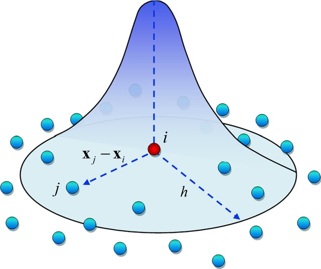
\includegraphics[width=\textwidth]{images/kernel.png}
                \caption*{ kernel function $\phi_h$}
            \end{figure}
        \end{column}
    \end{columns}
\end{frame}

\begin{frame}{An example: Vortex Method~\footnotemark[1]}
    \begin{columns}[t]
        \begin{column}{0.4\textwidth}
            \begin{itemize}
                \item incompressible Euler equation: particles discretize the \textbf{vorticity field} $\omega(x, t)$
                \item Particule strength $\Gamma_p$ is a local \textbf{circulation}
                \item Model evolution: \\
                      \begin{eqnarray*}
                          \frac{d\Gamma_p}{dt} &=& 0, \\
                          \frac{d x_p}{d t} &=& v(x_p; \mathcal P) \\
                          &=& \sum_{p' \in \mathcal P} \Gamma_{p'} \vec{V}(x_p - x_{p'}) + v_{BC} \\
                      \end{eqnarray*}
            \end{itemize}
            \footnotetext[1]{\tiny \cite{cottet_vortex_2000}}
        \end{column}
        \begin{column}{0.6\textwidth}
            \begin{figure}
                \centering
                \alt<2>{%
                    \animategraphics[loop, autoplay, width=0.7\textwidth]{5}{images/particles_ref/particles_ref_}{0}{20}
                }{%
                    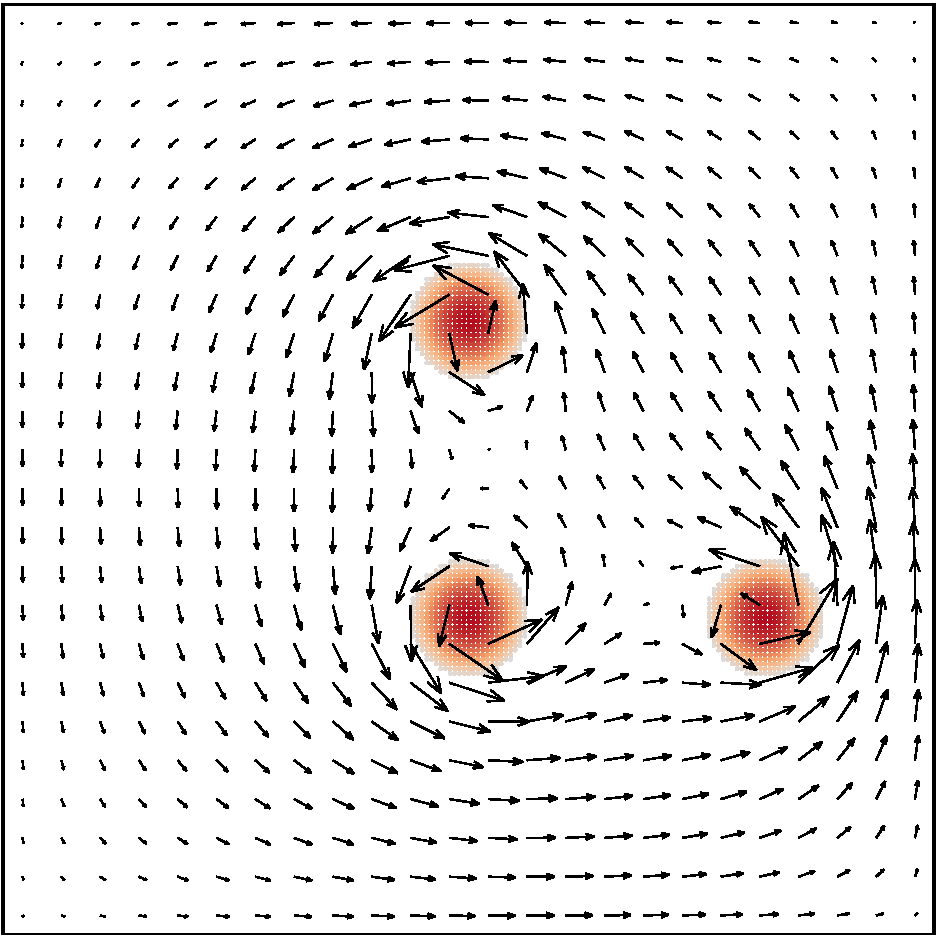
\includegraphics[width=0.7\textwidth]{images/particles_ref/particles_ref_0}%
                }
                \caption*{Three vortex problem}
            \end{figure}
        \end{column}
    \end{columns}

\end{frame}

\subsection{Data assimilation}
\begin{frame}{Data assimilation}
    \begin{figure}
        \centering
        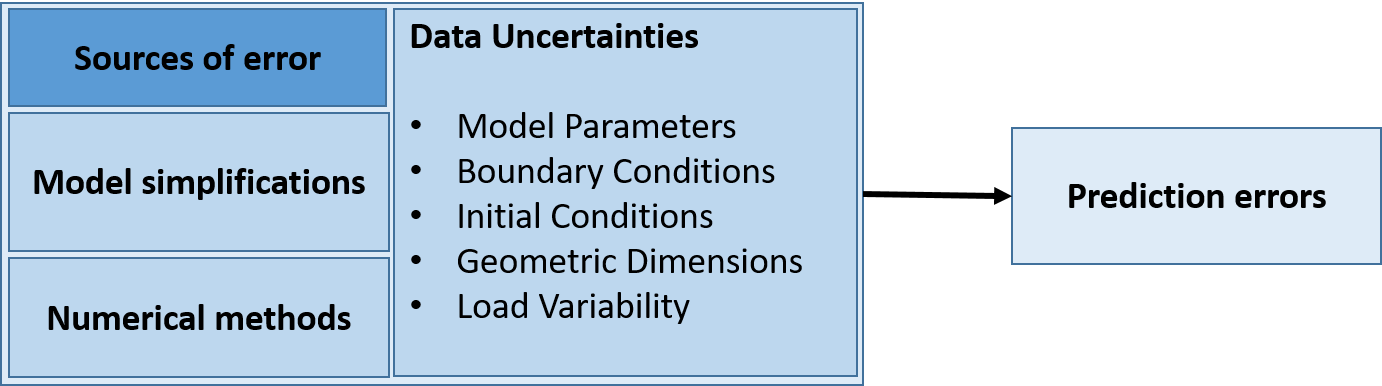
\includegraphics[width=0.7\textwidth]{images/source_of_uncertainties.png}
    \end{figure}

    \textbf{Goal:} Incorporate observations to reduce prediction error and uncertainties
    \begin{figure}
        \centering
        \alt<2>{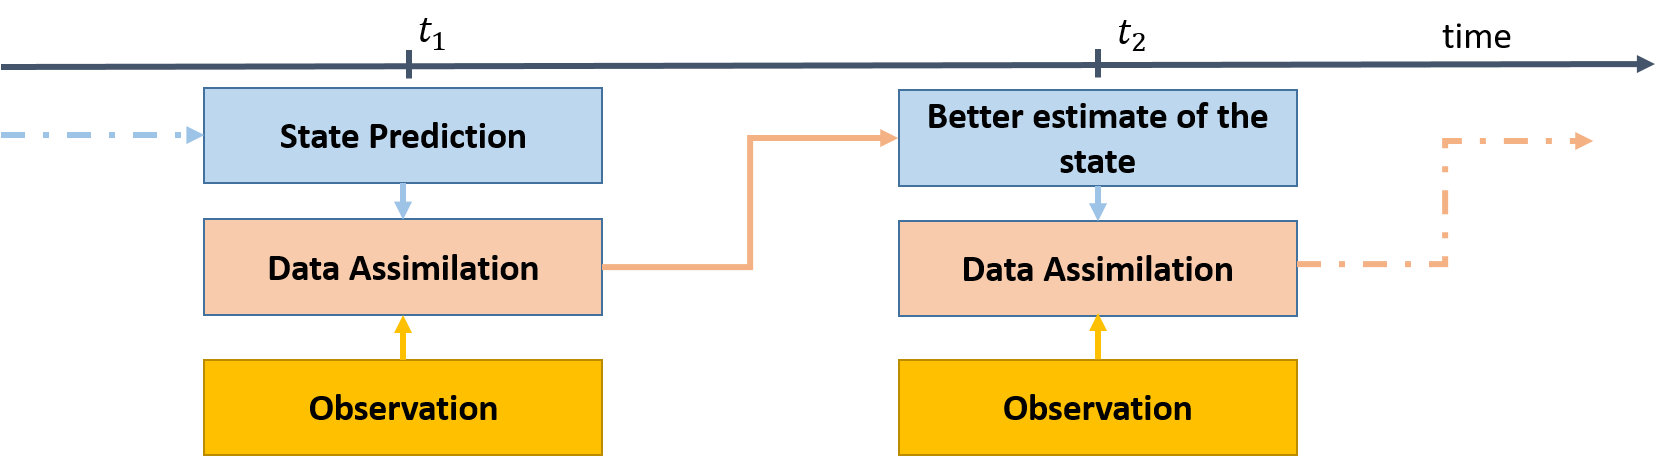
\includegraphics[width=0.8\textwidth]{images/da_scheme2.png}}{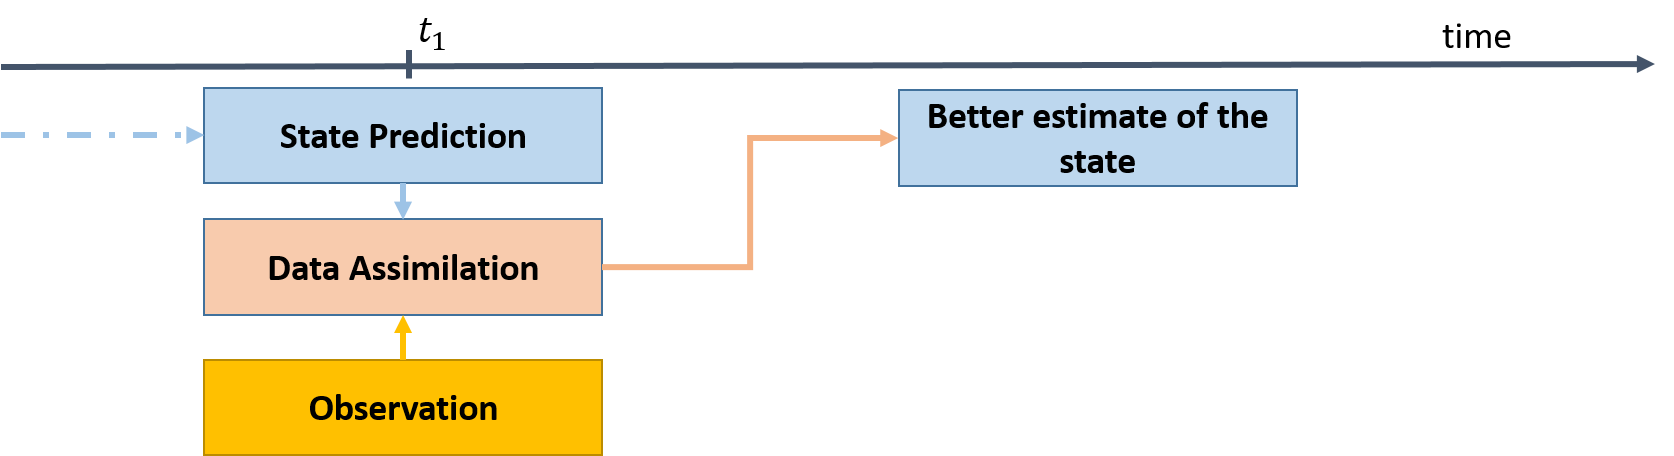
\includegraphics[width=0.8\textwidth]{images/da_scheme1.png}}
    \end{figure}

    \vfill
\end{frame}

\begin{frame}{Ensemble Kalman Filter}

    \begin{itemize}
        \item \textbf{Kalman Filter} extension with \textbf{ensemble} of members to estimate and propagate uncertainty of the state~\cite{evensen_sequential_1994}
        \item Adapted to \textbf{non-linear} and \textbf{high-dimensional} state space
    \end{itemize}
    \vspace{-0.4cm}
    \begin{columns}[t]
        \begin{column}{0.6\textwidth}
            \small

            \textbf{EnKF steps} (we note $u(\cdot, t_{k}) = u_k(\cdot)$):
            \begin{itemize}
                \item \textbf{Initialization}: \\
                      Sample $N_{\text{ens}}$ fields $\textcolor{blue}{\left\{u_{i,0}\right\}_{i=1}^{N_{\text{ens}}}} \stackrel{iid}{\sim} U_0$
                \item \textbf{Forecast}: from $t$ to $t_{k+1}$: \\
                      $\textcolor{blue}{ u^f_{i, k+1}} = \mathcal M(u_{i, k}), \quad i = 1, \dots, N_{\text{ens}}$
                \item \textbf{Measurement and prediction} at $t_{k+1}$:\\
                      measure $\textcolor{glycine}{y_{k+1}}$, \\
                      prediction $\textcolor{glycine}{h^i_{k+1}} = \mathcal H (\textcolor{blue}{ u^f_{i, k+1}}) \quad i = 1, \dots, N_{\text{ens}}$
                \item \textbf{Analysis}: a weighted linear combination of $u^f_{i,k+1}$ \\
                      $\textcolor{ceared}{u^a_{i, k+1}} = \textcolor{blue}{ u^f_{i, k+1}} + \sum_{j=1}^{N_{\text{ens}}} \textcolor{glycine}{\bm F_{ij}} \textcolor{blue}{ u^f_{j,k+1}}$, \\ where $\textcolor{glycine}{\bm F}$ depends on $\left(\textcolor{glycine}{y_{k+1}, \left\{h_{i, k+1}\right\}_{i=1}^{N_{\text{ens}}}}\right)$\footnotemark[1]
            \end{itemize}
            \vspace{0.25cm}

        \end{column}
        \begin{column}{0.4\textwidth}

            \begin{figure}[t]
                \centering
                \only<1>{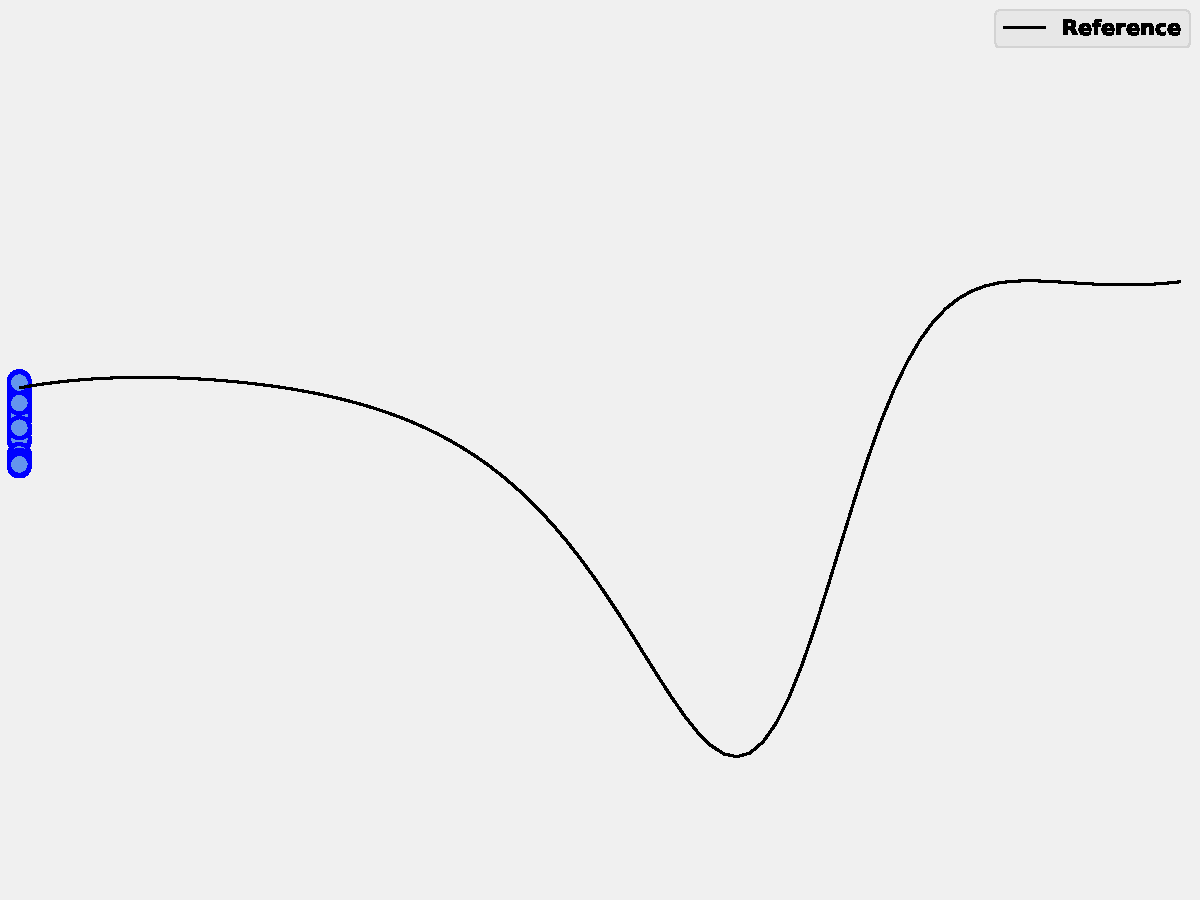
\includegraphics[width=\textwidth]{images/enkf_traj/enkf_lorenz_init.pdf}}
                \only<2>{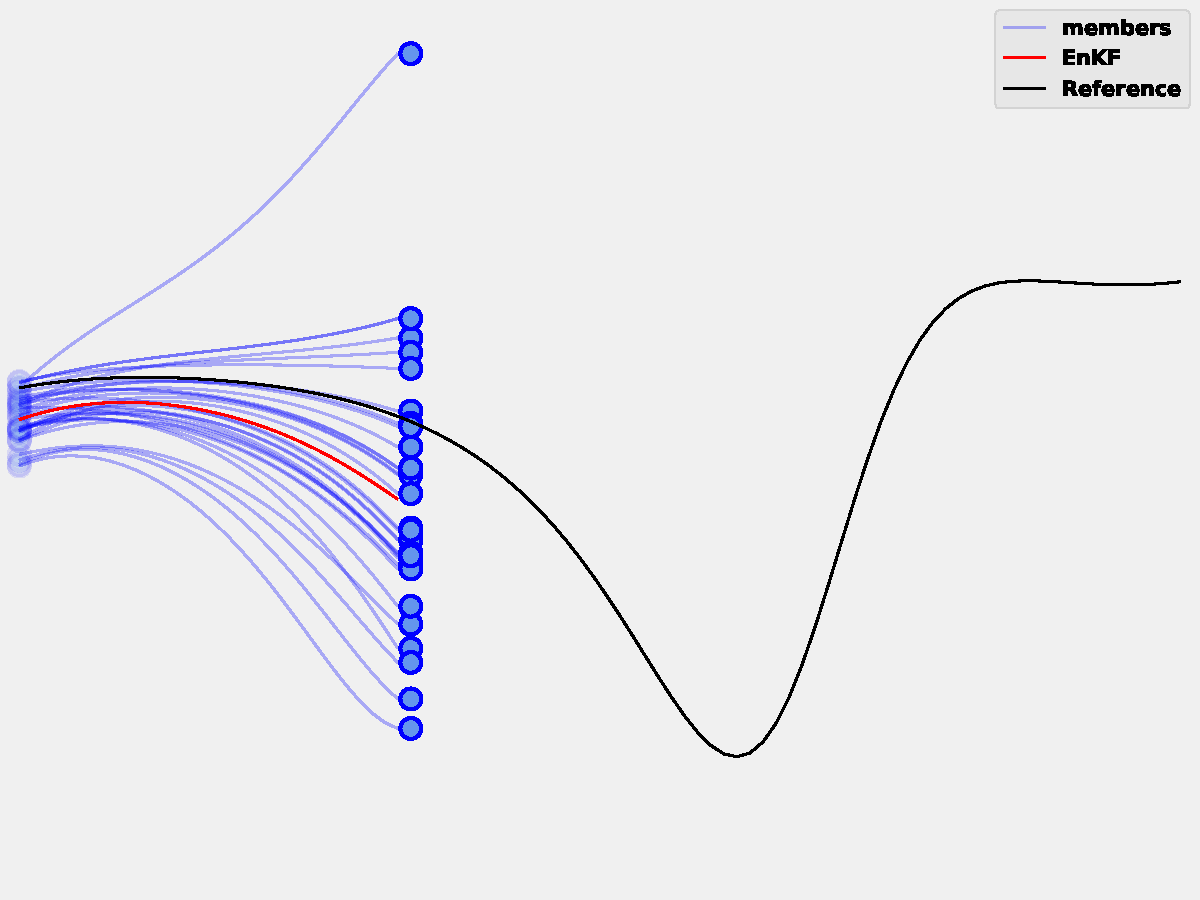
\includegraphics[width=\textwidth]{images/enkf_traj/enkf_lorenz_prop.pdf}}
                \only<3>{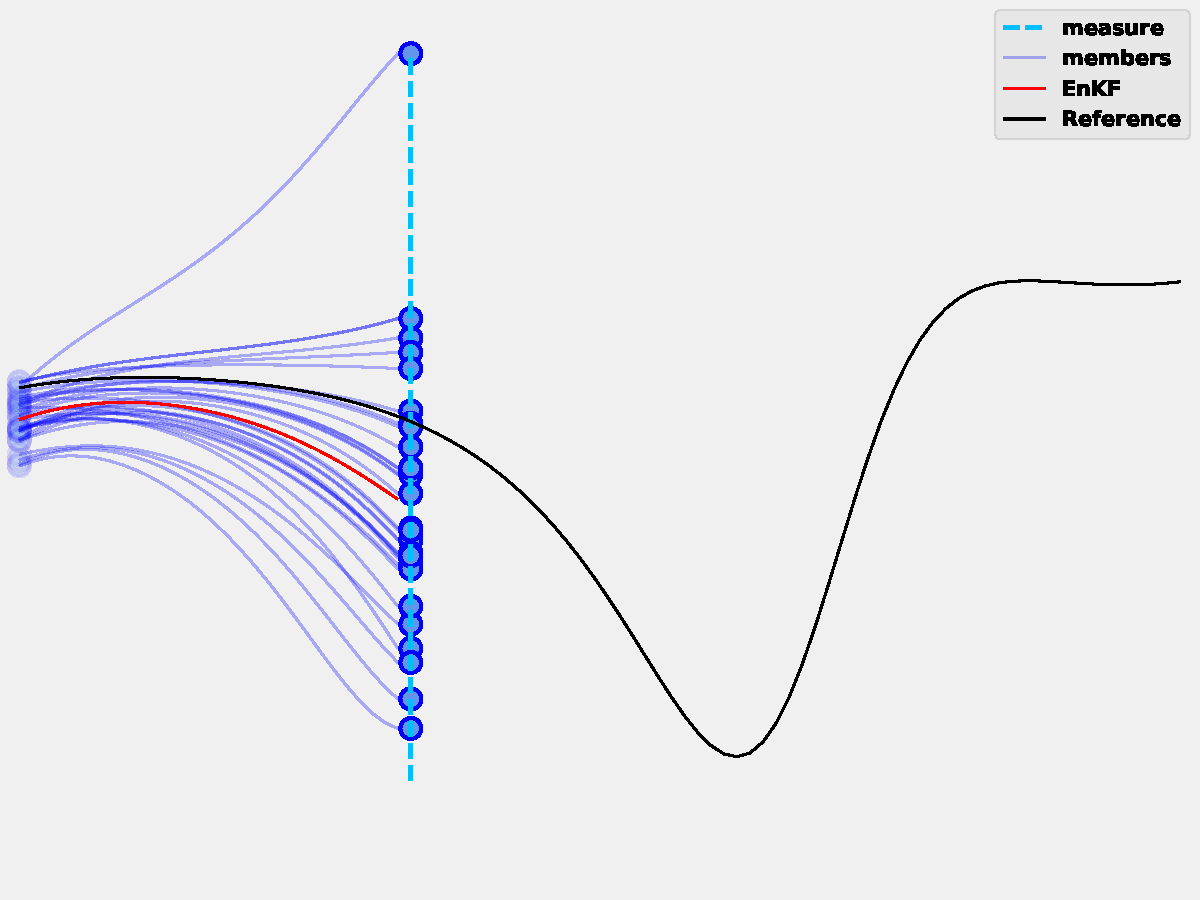
\includegraphics[width=\textwidth]{images/enkf_traj/enkf_lorenz_measure.pdf}}
                \only<4>{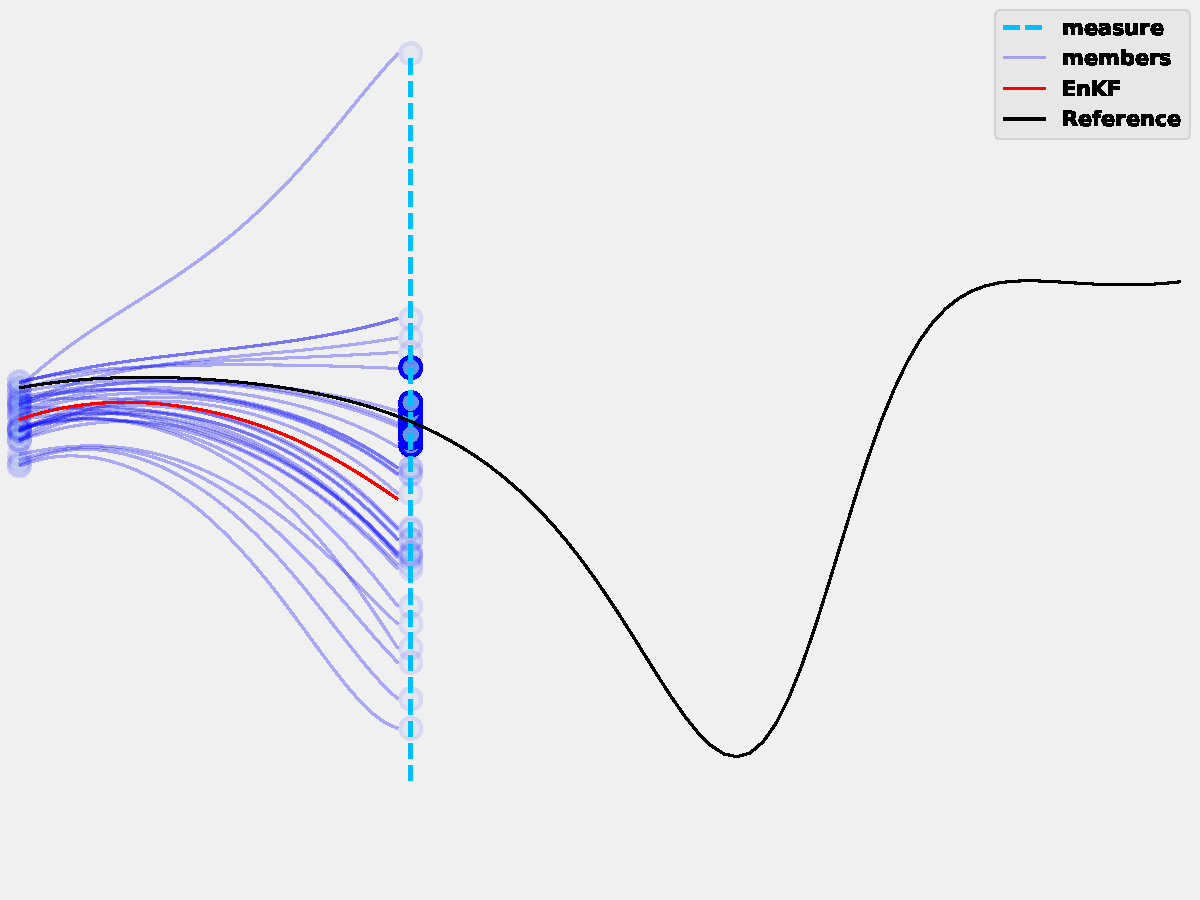
\includegraphics[width=\textwidth]{images/enkf_traj/enkf_lorenz_assim.pdf}}
                \only<5>{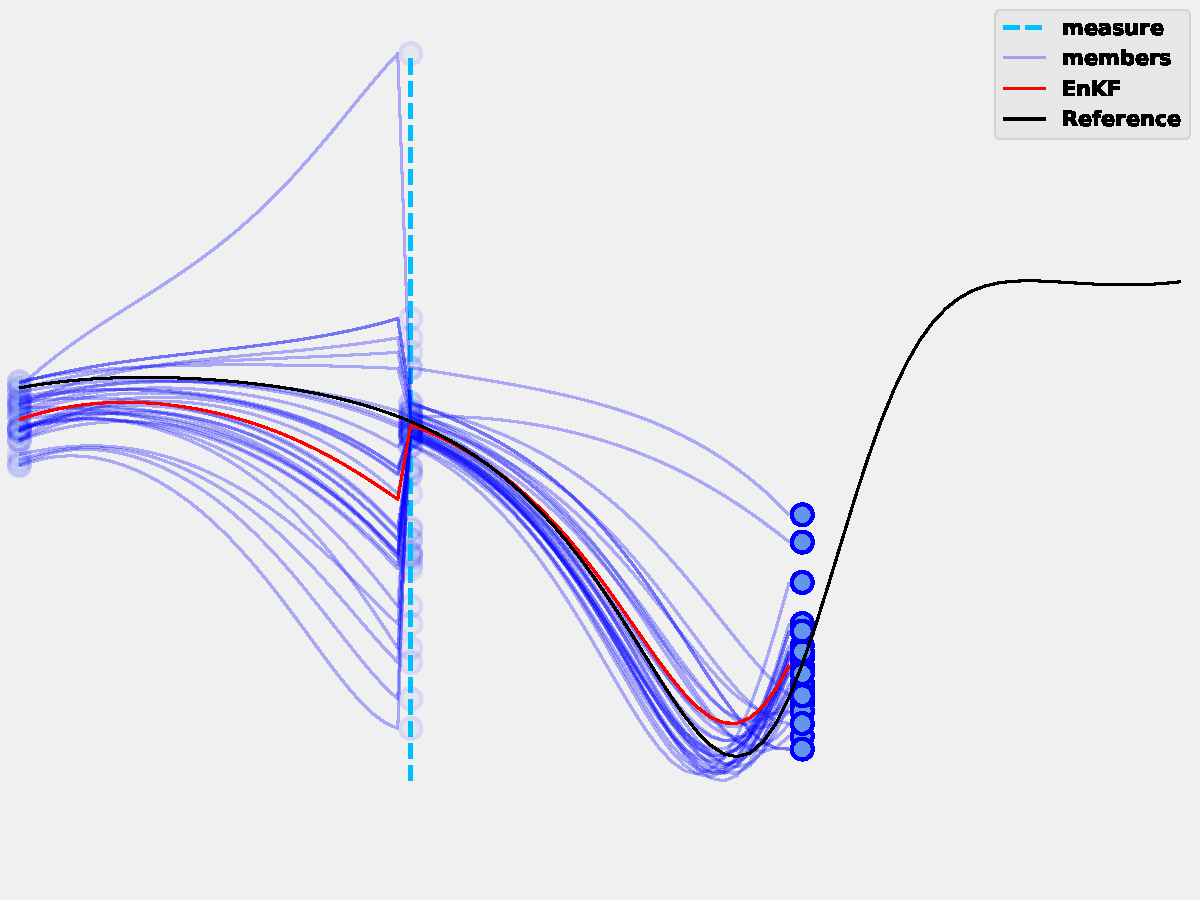
\includegraphics[width=\textwidth]{images/enkf_traj/enkf_lorenz_prop2.pdf}}
                \only<6>{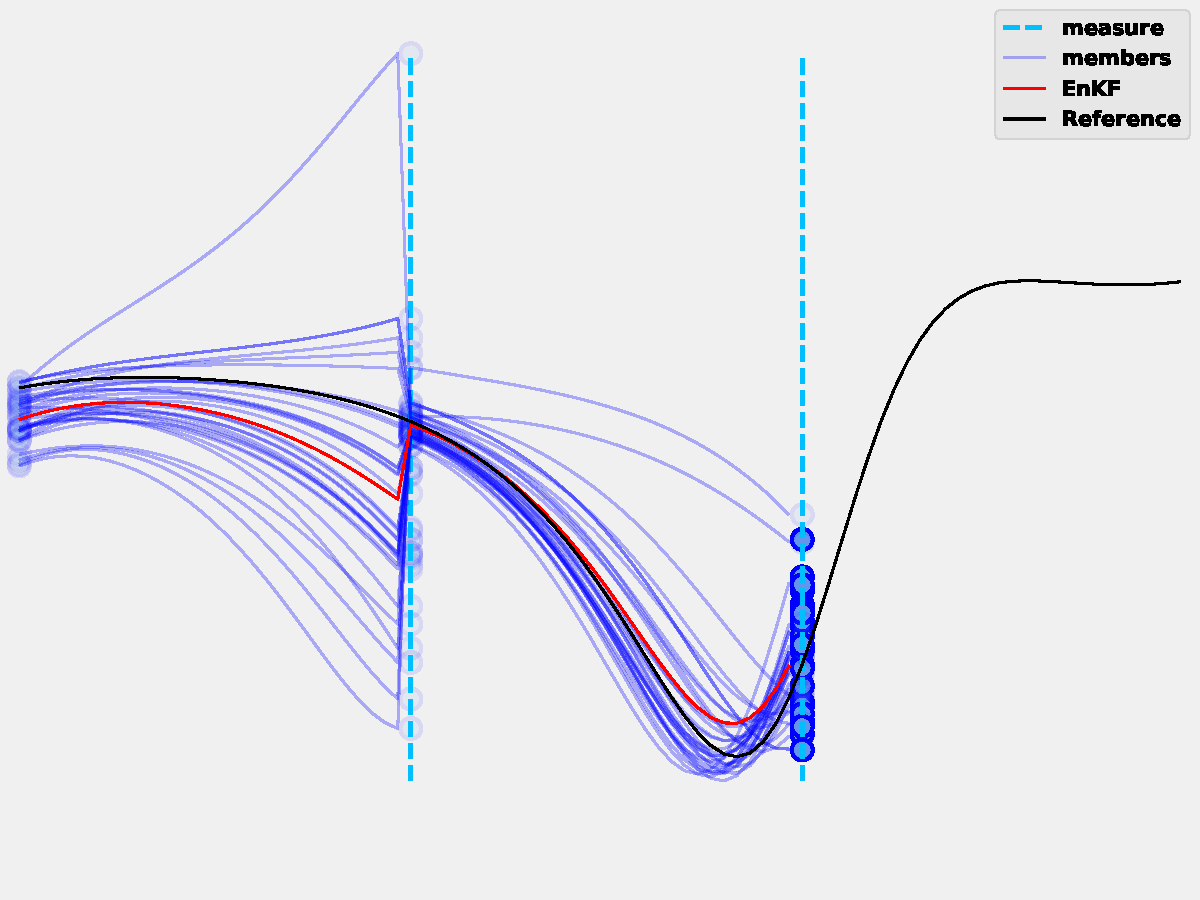
\includegraphics[width=\textwidth]{images/enkf_traj/enkf_lorenz_assim2.pdf}}
                \only<7->{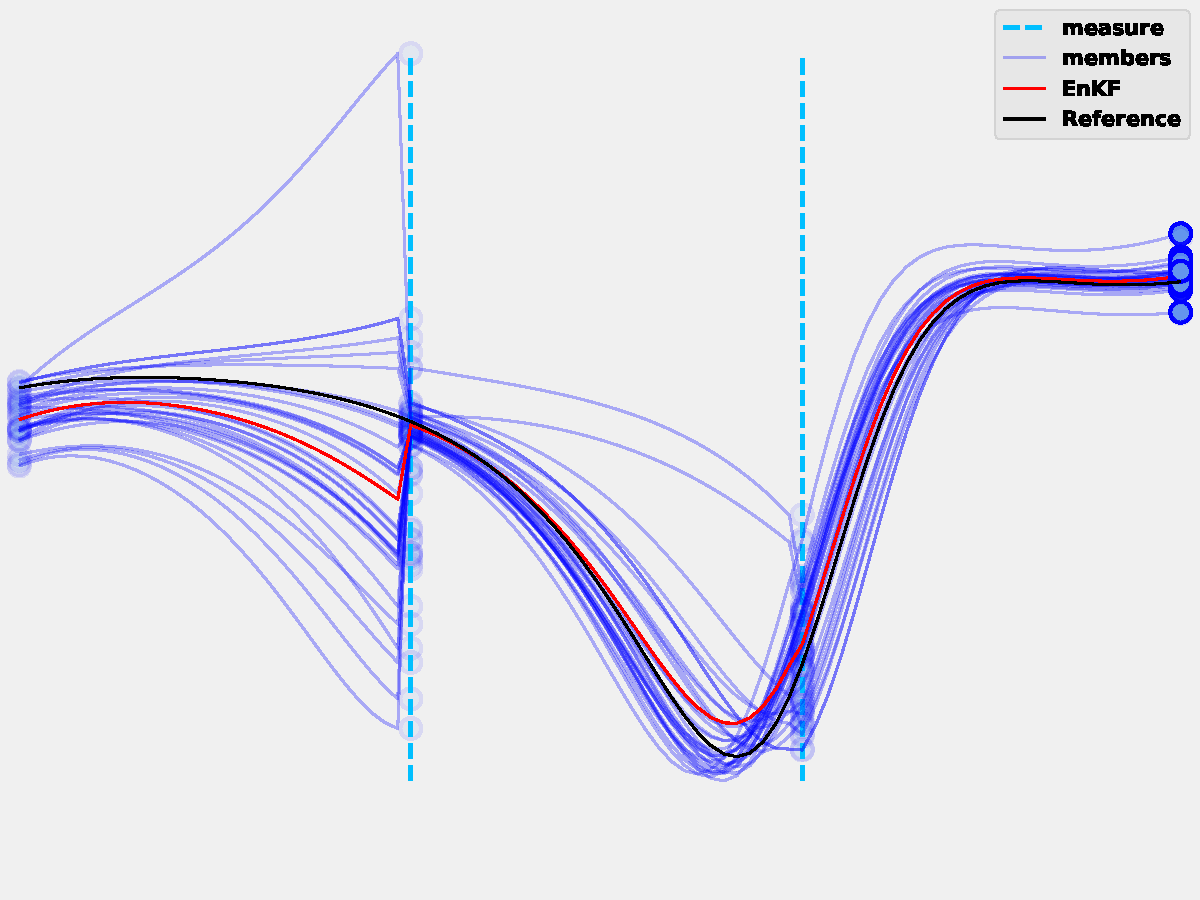
\includegraphics[width=\textwidth]{images/enkf_traj/enkf_lorenz_final.pdf}}
            \end{figure}
            \visible<8->{\textcolor{ceared}{\large How to apply this correction to meshless simulations ?}}
        \end{column}
    \end{columns}
    \vfill
    \footnotetext[1]{\tiny equivalent formulation of the original formulation, see~\cite{siripatana_combining_2019}}
\end{frame}

\transition[2]{Data assimilation for meshless simulations}{Strength correction}
\section{Data assimilation for meshless simulations}
\subsection{Strength correction}
\begin{frame}{EnKF Update for meshless simulations}

    \begin{columns}[t]
        \begin{column}{0.7\textwidth}
            Members correction $i = 1, \dots, N_{\text{ens}}$: \\
            \vspace{-0.50cm}
            \begin{eqnarray*}
                u_i^a(x) &=& u^f_i(x) + \sum_{j=1}^{N_{\text{ens}}} F_{ij}~u^f_j(x), \\
                &=& \sum_{p \in \mathcal{P}^f_i} \Gamma^f_p \phi_h(x - x_p) + \sum_{j=1}^{N_{\text{ens}}} F_{ij} \sum_{{p'} \in \mathcal{P}_j^f} \Gamma^f_{p'} \phi_h(x - x_{p'}), \\
                &=& \sum_{j=1}^{N_{\text{ens}}} \sum_{ p \in \mathcal{P}^f_i} \Gamma^a_p \phi_h (x - x_p)
            \end{eqnarray*}
            \vspace{-0.10cm}
            $\Rightarrow u_i^a$ is a combinaison of \textbf{all particles}! \\
            \vspace{-0.10cm}
            \begin{equation*}\text{Card}(\mathcal P^a_i) = \sum_{j=1}^{N_{\text{ens}}}\text{Card}(\mathcal P^f_j)
            \end{equation*}
        \end{column}
        \begin{column}{0.3\textwidth}
            \vspace{-1cm}
            \begin{figure}
                \centering
                \begin{subfigure}{\textwidth}
                    \centering
                    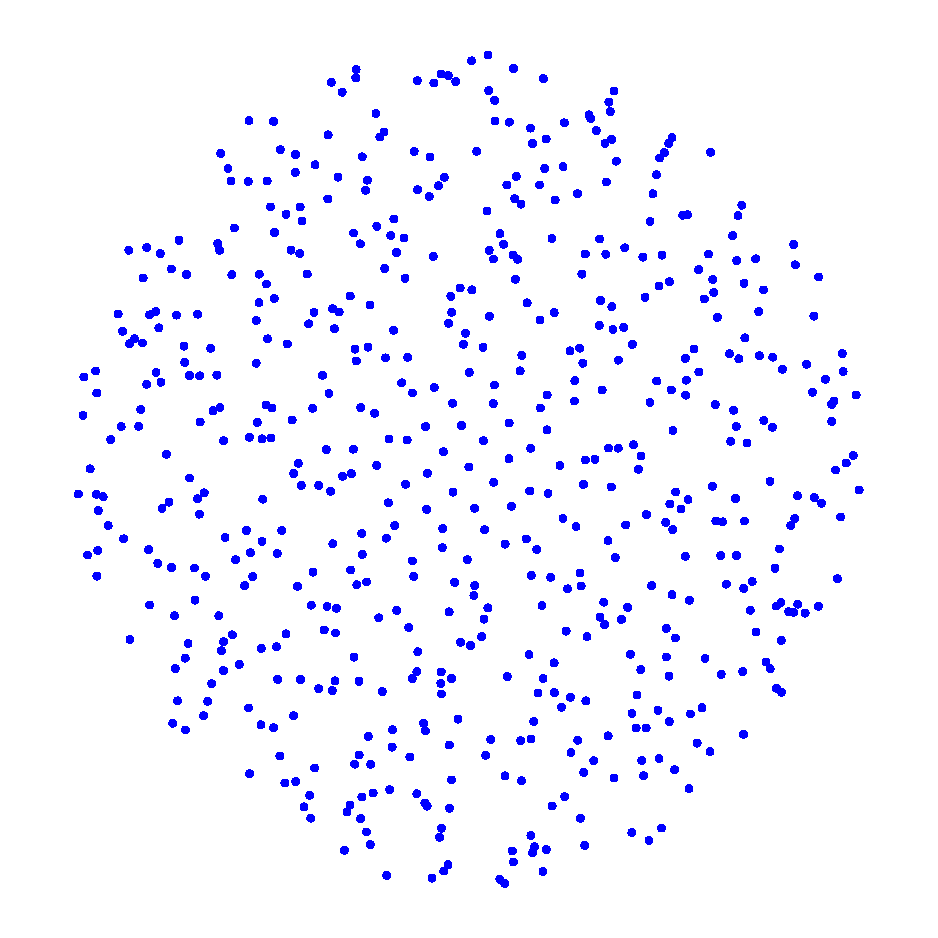
\includegraphics[width=0.7\textwidth]{images/memb_particles.pdf}
                \end{subfigure}
                \begin{subfigure}{\textwidth}
                    \centering
                    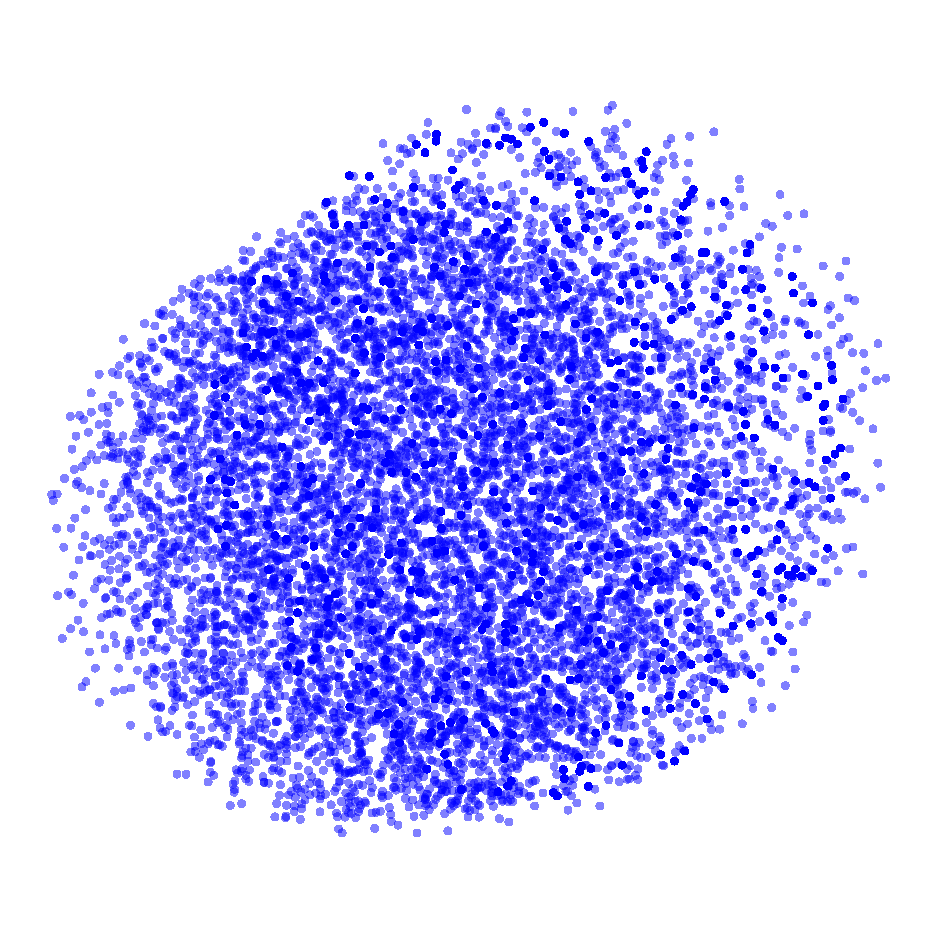
\includegraphics[width=0.7\textwidth]{images/all_particles.pdf}
                \end{subfigure}
                \caption*{Particle support before and after the correction}
            \end{figure}
        \end{column}
    \end{columns}
\end{frame}

\begin{frame}{Strength correction}
    \small
    \textbf{Solution 1} \\
    Generate a new regular particle set with particle-grid operator~\footnotemark[1] \\
    \vspace{0.5cm}
    \textbf{Solution 2} \\
    \begin{columns}[t]
        \begin{column}{0.5\textwidth}
            Keep the same set of particle positions
            \begin{eqnarray*}
                u_i^f(x) &=& \sum_{p \in \mathcal P_i} \textcolor{ceared}{\Gamma^f_p} \phi_h(x - x_p^f),\\
                u_i^a(x) &\approx& \sum_{p \in \mathcal P_i} \textcolor{ceared}{\Gamma^a_p} \phi_h(x - x_p^f), \\
                % \left\{x^f_{p}, \hat \Gamma^f_{p}\right\}_{p=1}^{N^i_p} \mapsto \left\{x_{p}, \textcolor{ceared}{\langle u^i, \phi_h(\cdot,x_{p})\rangle} \right\}_{p=1}^{N_p^i}
            \end{eqnarray*}where $\textcolor{ceared}{\Gamma^a_p} = \langle u^a_i, \phi_h(\cdot,x_{p})\rangle$
        \end{column}
        \begin{column}{0.5\textwidth}
            Confined to the particle support $\rightarrow$ might be inadequate for the analyzed solution
            \begin{figure}
                \centering
                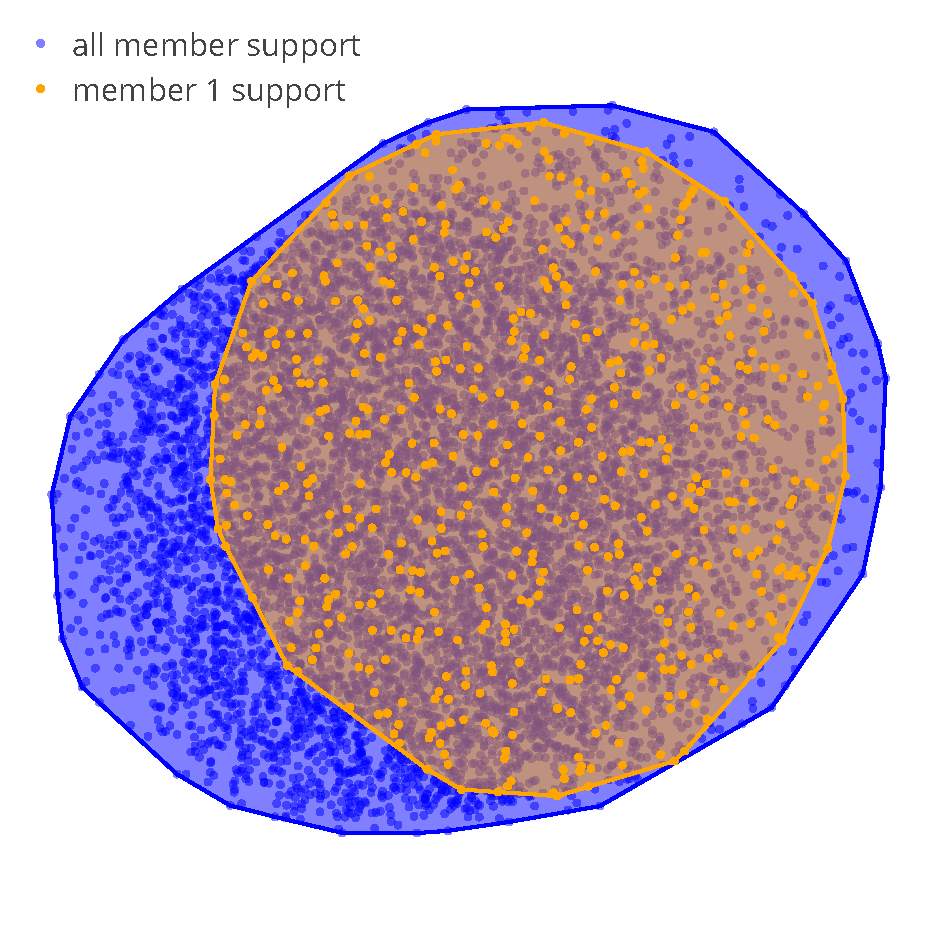
\includegraphics[width=0.6\textwidth]{./images/ens_particles.pdf}
            \end{figure}
        \end{column}
    \end{columns}
    \vfill
    \footnotetext[1]{\tiny used by particles-in-cell methods (MPM, VIC,...).}
\end{frame}

\transition[3]{Data assimilation by alignment}{Position correction}
\subsection{Position correction}
\begin{frame}{Position correction}
    \vspace{-0.9cm}
    \begin{eqnarray*}
        u_i^f(x) &=& \sum_{p \in \mathcal P_i} \Gamma^f_p \phi_h(x - \textcolor{ceared}{x_p^f}), \quad u^a_i(x) = u_i^f(x) + \sum_{j=1}^{N_{\text{ens}}} F_{ij} u_j^f(x), \\
        u_i^a(x) &\approx& \sum_{p \in \mathcal P_i} \Gamma^f_p \phi_h(x - \textcolor{ceared}{A_i(x_p^f)}), \\
    \end{eqnarray*}
    \vspace{-0.7cm}

    \begin{columns}[t]
        \begin{column}{0.6\textwidth}
            $A_i$ is a mapping such as $x^a_{p} = A_i(x^f_{p})$. \\
            Here we choose~\footnotemark[1] to write $A(x)$ as the solution of\\
            \begin{equation*}
                \begin{cases}
                    x'(\tau = 0) = x,                                           \\
                    \frac{d x'}{d \tau} = w_i (x'), \quad A_i(x) = x'(\tau = 1) \\
                \end{cases}
            \end{equation*}with $w_i$ a velocity field \textbf{to determined}
        \end{column}
        \begin{column}{0.4\textwidth}
            \vspace{-2cm}
            \begin{figure}
                \centering
                \only<1>{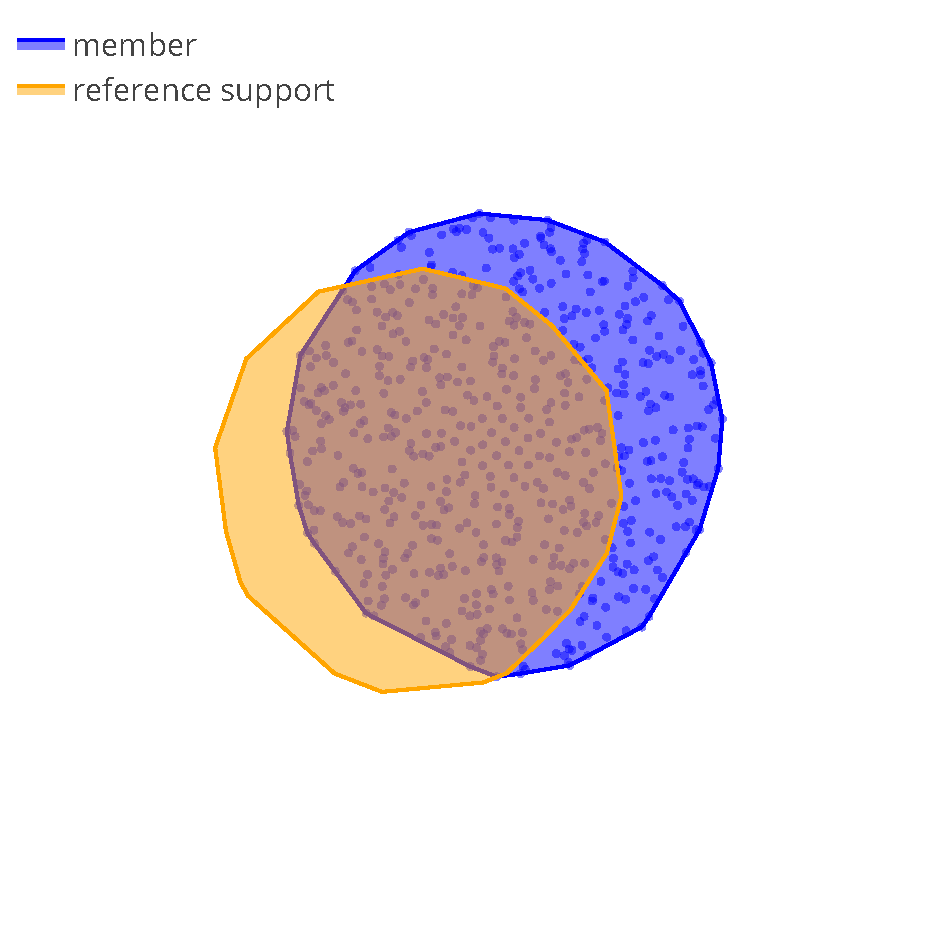
\includegraphics[width=0.8\textwidth]{images/align_member_0.pdf}}
                \only<2>{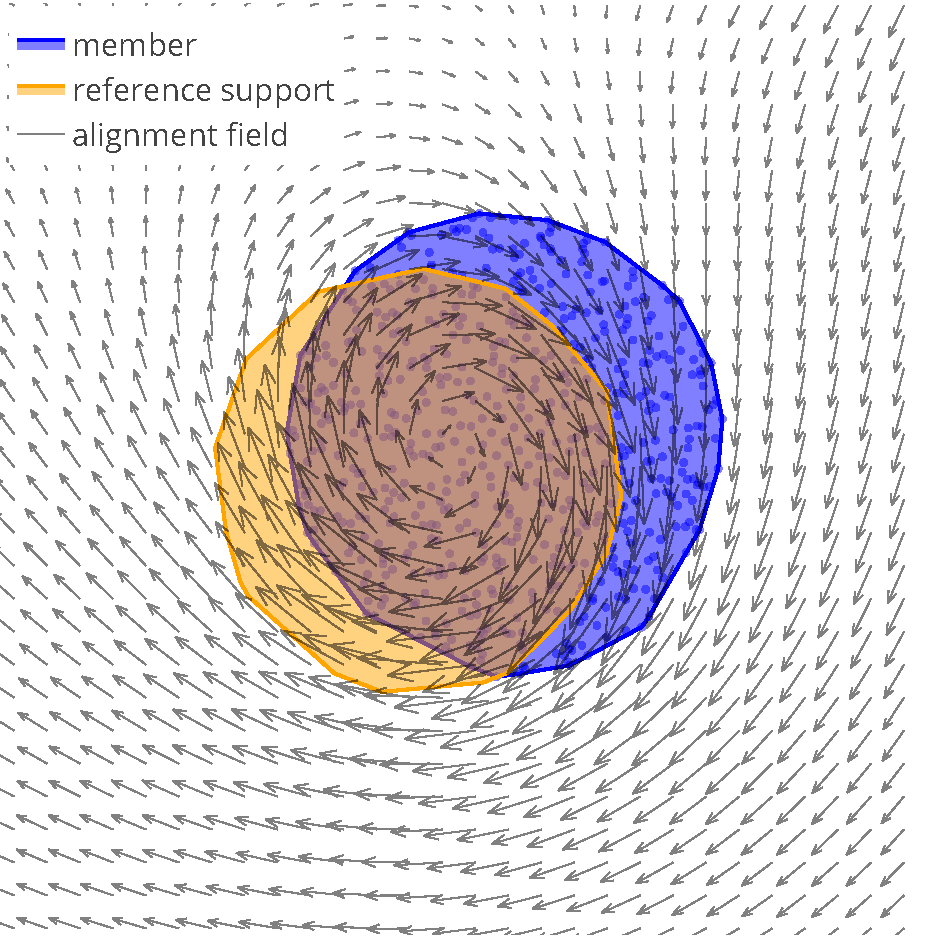
\includegraphics[width=0.8\textwidth]{images/align_member_1.pdf}}
                \only<3>{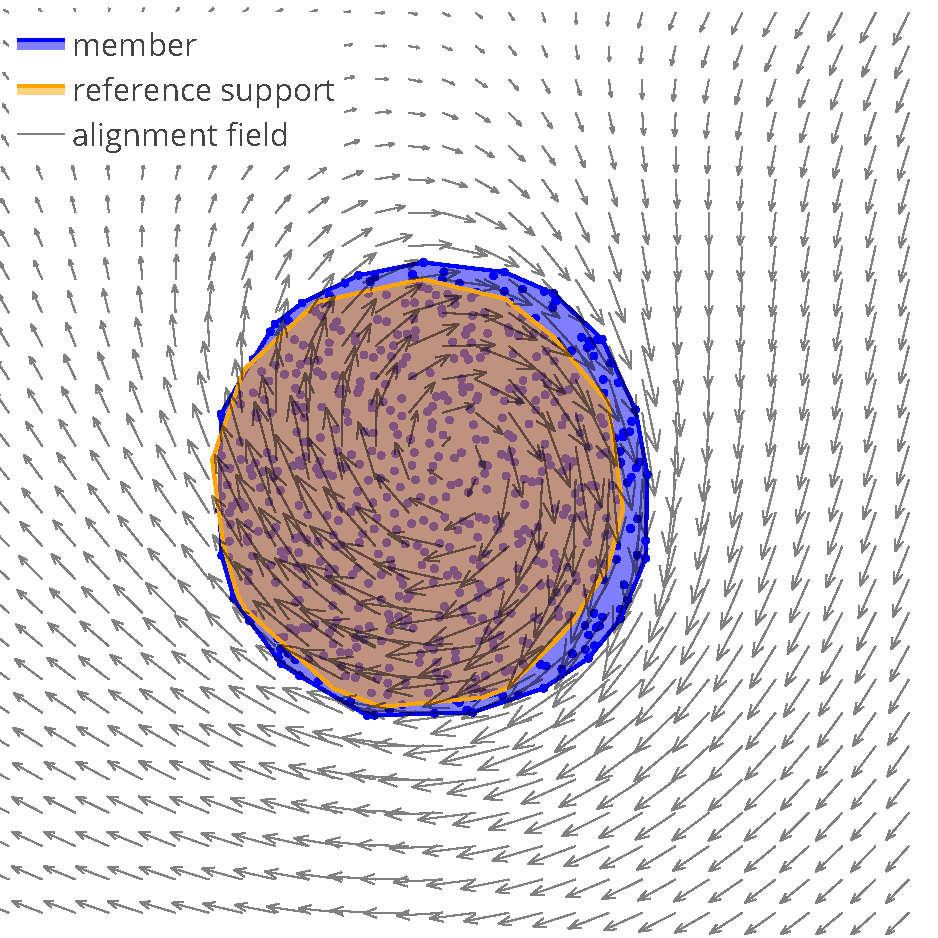
\includegraphics[width=0.8\textwidth]{images/align_member_2_1.pdf}}
            \end{figure}
        \end{column}
    \end{columns}
    \vfill
    \footnotetext[1]{\tiny Other hypothesis have been made see~\cite{ravela_data_2007,rosenthal_displacement_2017}}
\end{frame}

\begin{frame}{Choose of $w_i$}
    For member $i$, we seek to reduce the discrepancy between \textbf{predictions} and the \textbf{observations}:
    \begin{equation*}
        w_i = \argmin_{w_i \in \mathcal V} \left\|y - \mathcal H(\mathcal{P}_i^f \mid w_i) \right\|^2 \visible<2->{\textcolor{ceared}{+ R(w)}}, \quad i = 1, \dots, N_{\text{ens}}
    \end{equation*}with $\mathcal V$ the velocity search space, $\mathcal H(\mathcal{P}_i^f \mid w_i)$ the observation operator conditioned by $w_i$\\
    \vfill
    \visible<2->{\textcolor{ceared}{$R(w)$} is a regularisation term (avoid non-uniqueness and ill-conditioning)\\}
    \vfill
    \visible<2->{\textbf{Infinite}-dimensional problem}
    \vfill
\end{frame}

\begin{frame}{Reduced order formulation}

    We search the velocity as a linear combination of member velocity fields,\\
    find $\bm a_i \in \mathbb{R}^{N_{\text{ens}}}$ \\
    \begin{equation*}
        w_i = \sum_{j=1}^{N_{\text{ens}}} a_{i,j} v_j (x) = \sum_{j=1}^{N_{\text{ens}}} a^i_j \left(\sum_{p \in \mathcal P_j} \Gamma_p^f \vec{V}(x - x_p) + v_{j,BC} \right)
    \end{equation*}
    \vfill
    \visible<2->{Leads to $N_{\text{ens}}$ independent problems of dimension $N_{\text{ens}}$ \\
        \begin{equation*}
            \mathcal L_i (a) = \min_{a \in \mathbb{R}^{N_{\text{ens}}}} \left\|d - \mathcal H_a(\hat u^f_i; a)_2 \right\|^2 + \lambda \|a\|_2^2, \quad i = 1, \dots, N_{\text{ens}}
        \end{equation*}
        Optimize with a local gradient optimizer (BFGS)}
    \vfill

\end{frame}

\transition[3]{Application}{Three vortex problem}

\section{Application}

\begin{frame}{Test problem - Three vortex(body) problem}
    \vspace{-0.5cm}
    \begin{columns}[t]
        \begin{column}{0.45\textwidth}
            \begin{itemize}
                \item \scriptsize \textbf{Variables of interest}: positions of vortex centers
                \item \scriptsize \textbf{Initial Uncertainties}: vortex mean positions, strength, core-size,...
                \item \scriptsize \textbf{chaotic trajectories}~\footnotemark[1]
                \item \scriptsize \textbf{observations}: a noisy coarse velocity grid
            \end{itemize}
            \begin{figure}
                \centering
                \vspace{-0.25cm}
                % \only<2->{\caption*{\tiny Vortex normalized position error}}
                \includegraphics<3->[width=\textwidth]{images/error_position_wo_assim.pdf}
            \end{figure}
            \vfill
        \end{column}
        \begin{column}{0.55\textwidth}
            \centering
            \begin{figure}[t]
                \centering
                \visible<2->{\tiny Vortex center trajectories for perturbed inputs}
                \only<3->{%
                    \animategraphics[loop, autoplay, width=0.85\textwidth]{10}{images/vortex_centers_disperse/vortex_centers_}{0}{36}%
                }
                \only<2>{%
                    \animategraphics[loop, autoplay, width=0.85\textwidth]{10}{images/vortex_centers_ref/vortex_centers_}{0}{36}
                }
                \only<1>{%
                    \animategraphics[loop, autoplay, width=0.7\textwidth]{5}{images/particles_ref/particles_ref_}{0}{20}
                }
            \end{figure}

        \end{column}
    \end{columns}
    \vspace{-0.5cm}

    \footnotetext[1]{\tiny \cite{aref_motion_1979}}
\end{frame}

\begin{frame}{Strength correction}
    \begin{columns}[t]
        \begin{column}{0.5\textwidth}
            \vspace{-0.5cm}
            \begin{figure}
                \centering
                \animategraphics[loop, autoplay, width=\textwidth]{10}{images/vortex_centers_part_enkf/vortex_centers_}{0}{36}
            \end{figure}
        \end{column}
        \begin{column}{0.5\textwidth}
            \begin{figure}
                \centering
                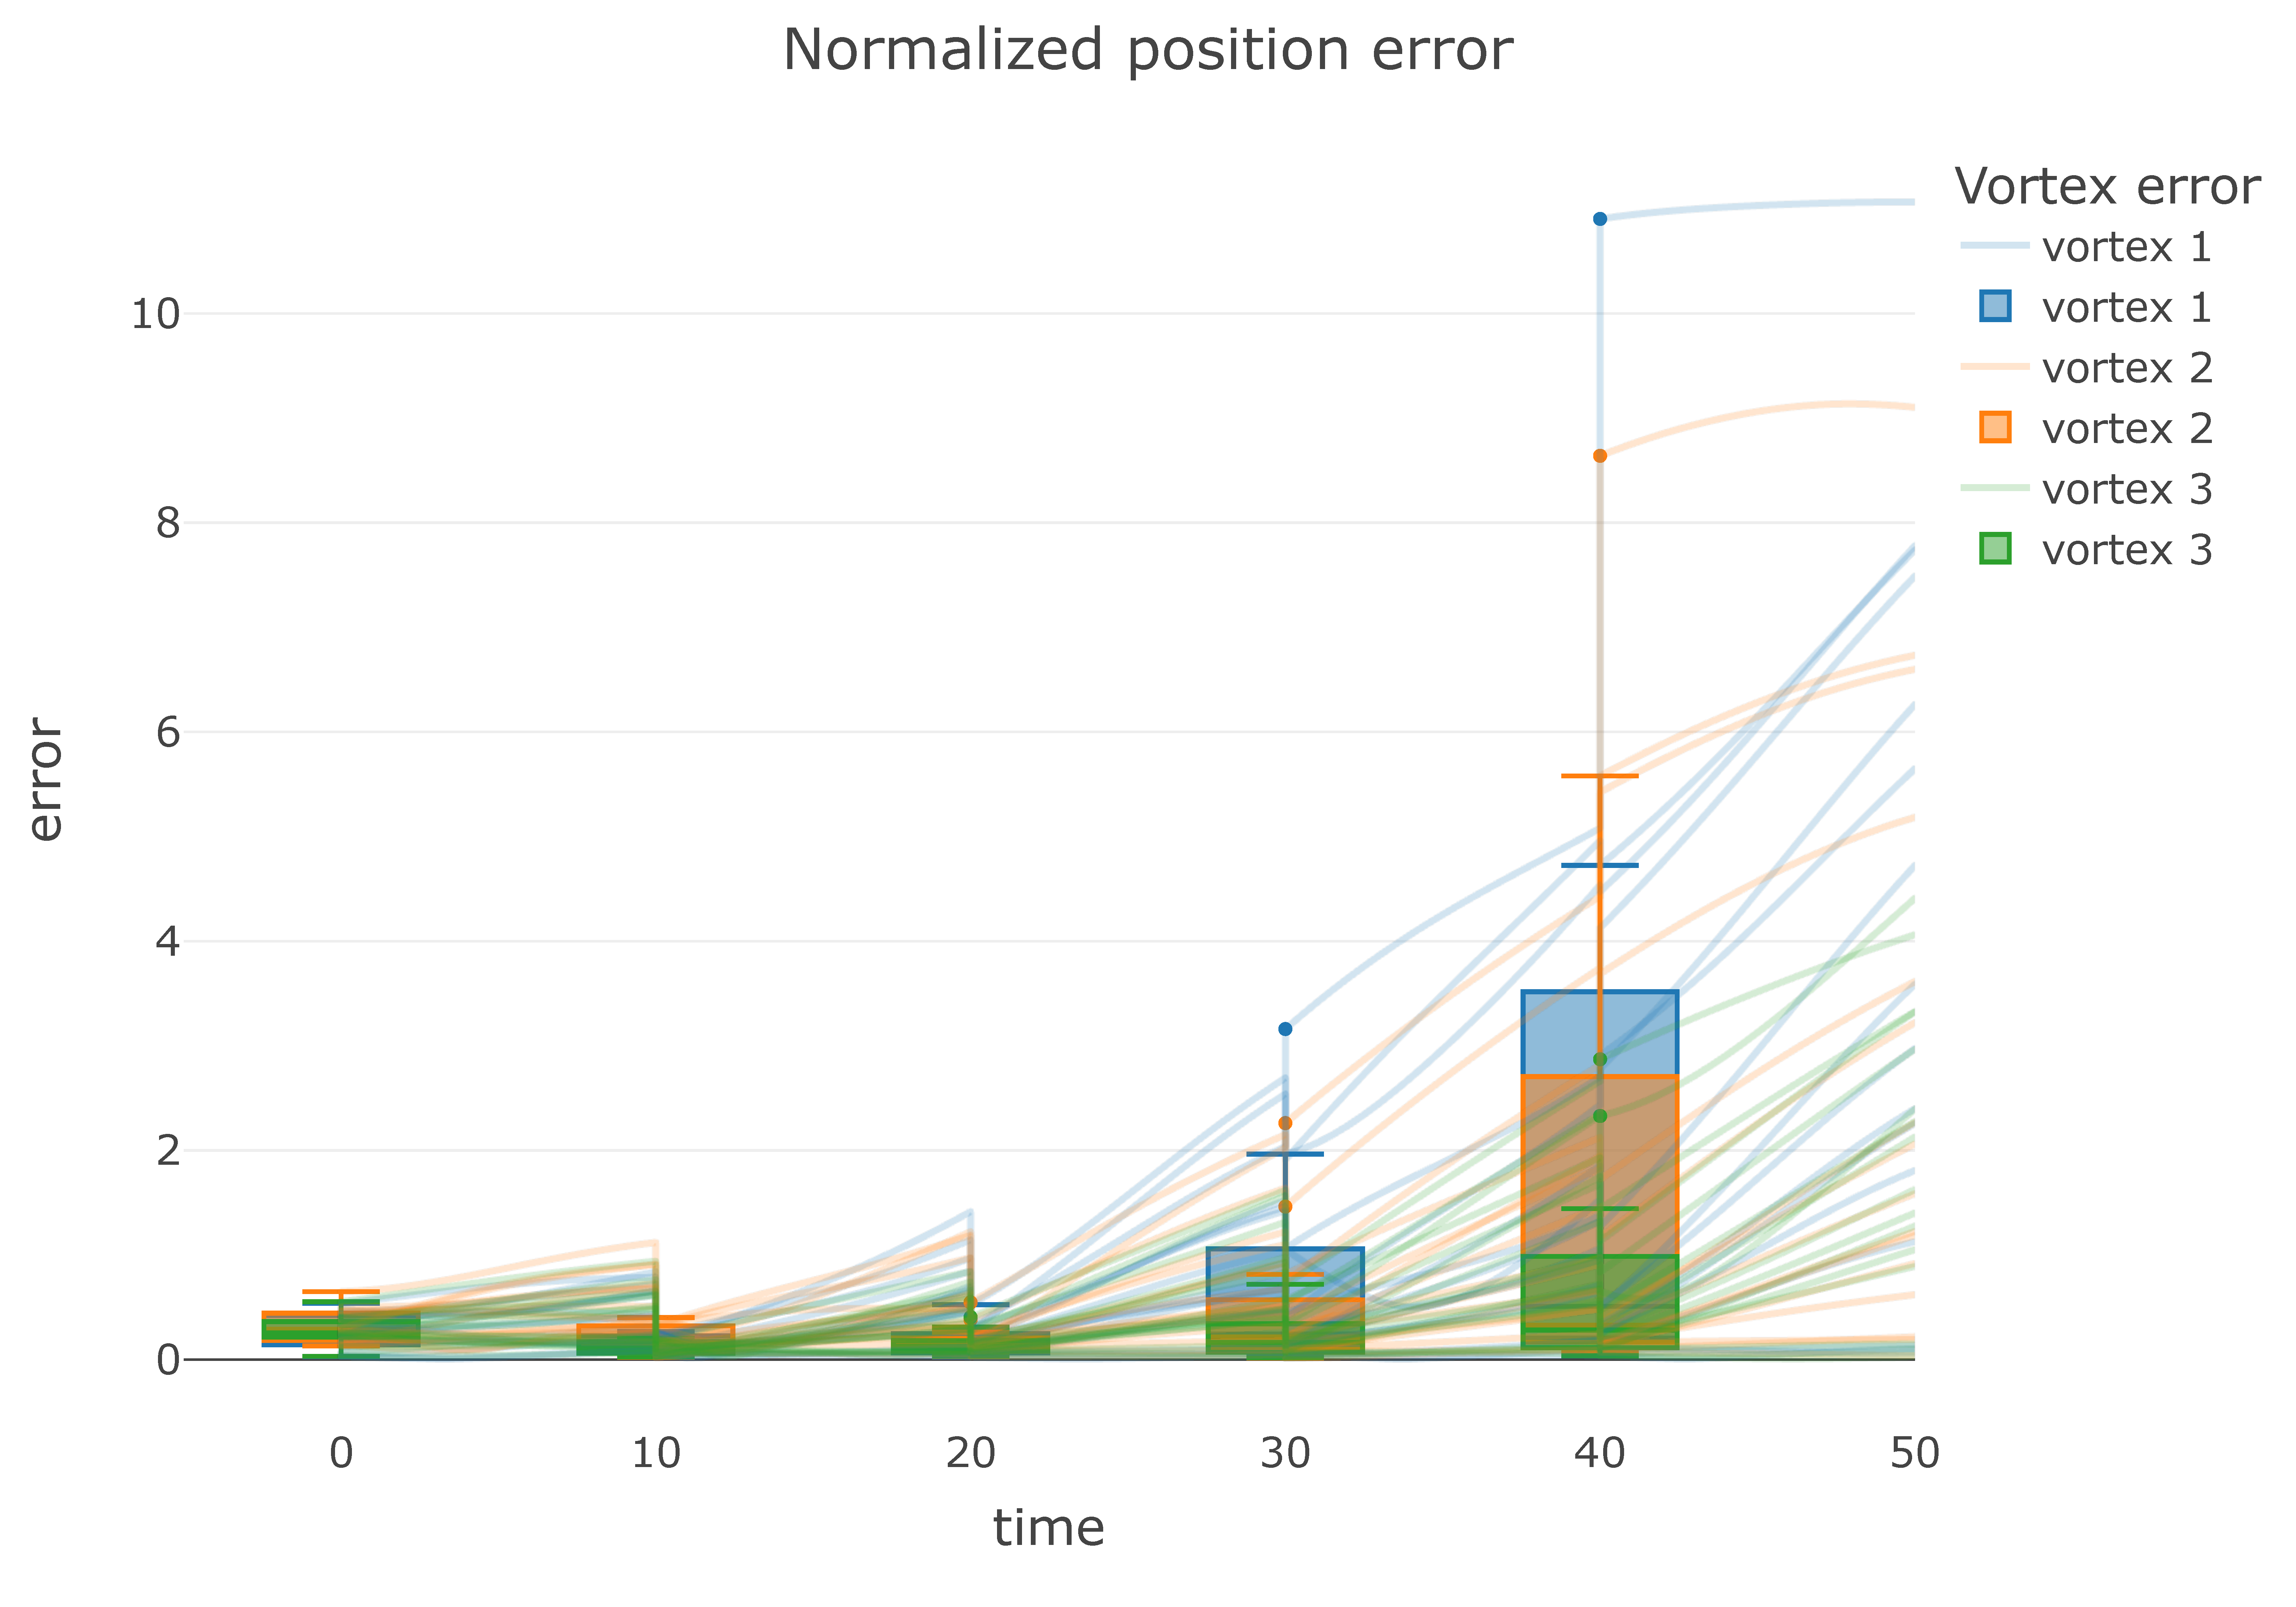
\includegraphics[width=\textwidth]{images/part_enkf_error.pdf}
            \end{figure}

            \begin{itemize}
                \item \textbf{not a convinent case} to apply strength correction
            \end{itemize}
        \end{column}
    \end{columns}
\end{frame}

\begin{frame}{Alignment correction}
    \vspace{-0.5cm}
    \begin{columns}[c]
        \begin{column}{0.45\textwidth}
            \begin{figure}
                \centering
                \caption*{\tiny Field alignment of member one at first assimilation step.}
                \includegraphics<1>[width=\textwidth]{images/align_member/align_member_prior.pdf}
                \includegraphics<2>[width=\textwidth]{images/align_member/align_member_prior_field.pdf}
                \includegraphics<3->[width=\textwidth]{images/align_member/align_member_final.pdf}
            \end{figure}

        \end{column}
        \begin{column}{0.55\textwidth}
            \begin{figure}[c]
                \centering
                \caption*{\tiny Vorticity field correction at first assimilation step.}
                \begin{subfigure}{0.49\textwidth}
                    \centering
                    \includegraphics<1-2>[width=\textwidth]{images/vorticity_prior.pdf}
                    \only<1-2>{\caption*{\tiny Before alignment}}
                    \includegraphics<3>[width=\textwidth]{images/vorticity_align.pdf}
                    \only<3>{\caption*{\tiny After alignment}}
                \end{subfigure}
                \begin{subfigure}{0.49\textwidth}
                    \centering
                    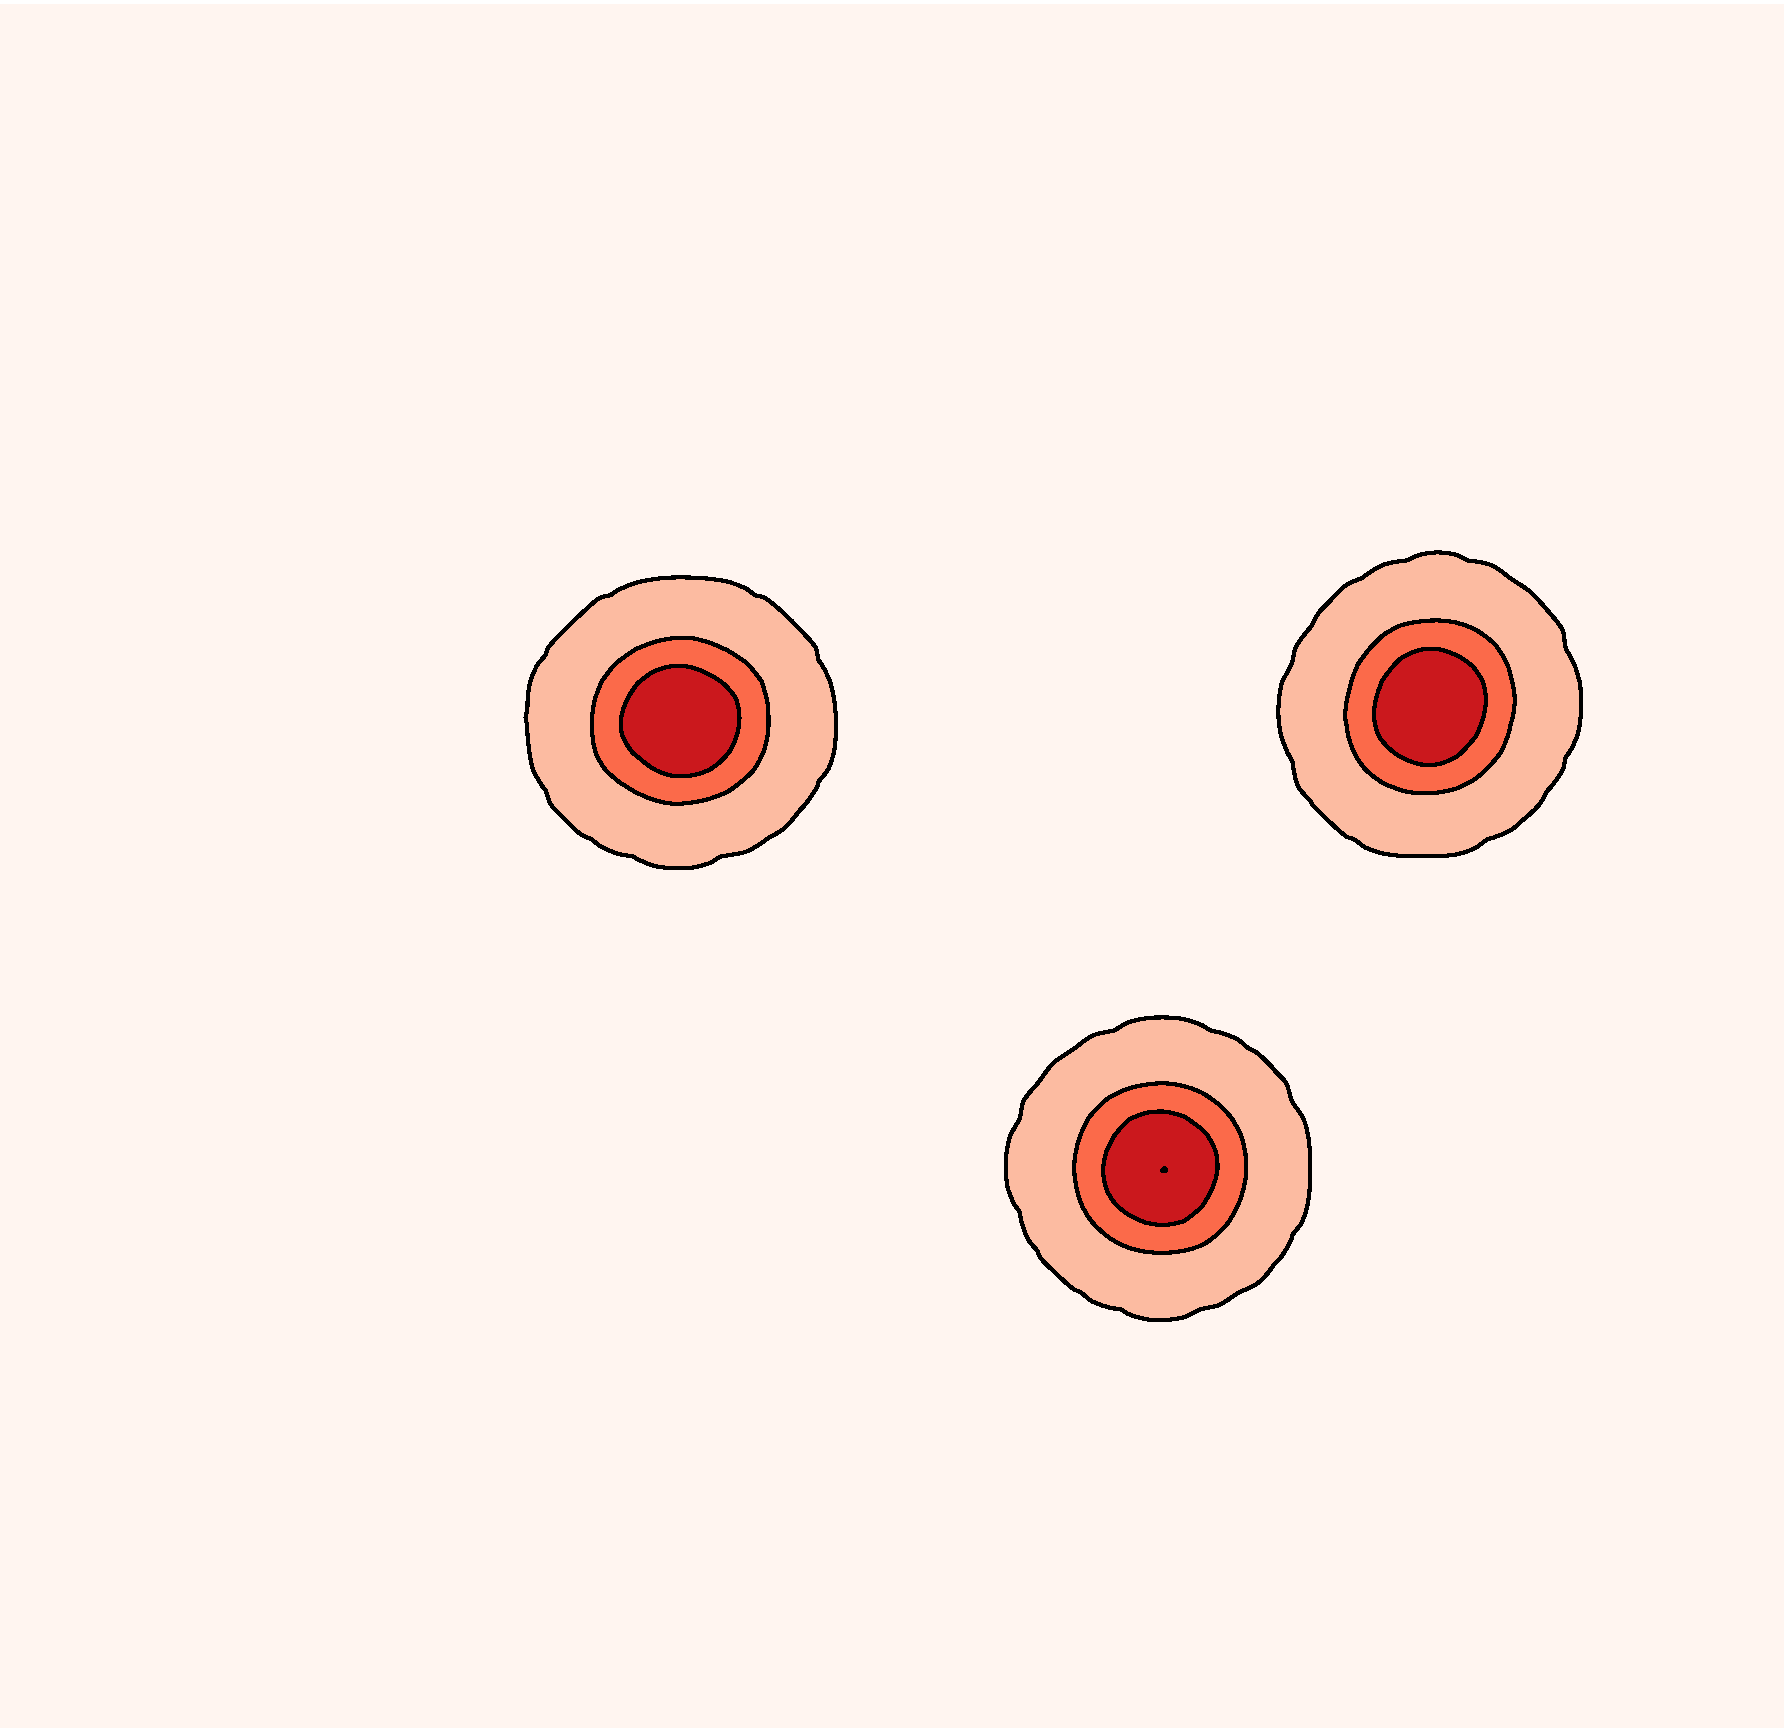
\includegraphics[width=\textwidth]{images/vorticity_ref.pdf}
                    \caption*{\tiny Reference}

                \end{subfigure}
            \end{figure}
        \end{column}
    \end{columns}

    \vspace{-0.25cm}

    \vspace{-0.25cm}
\end{frame}


\begin{frame}{Alignment correction}
    \vspace{-0.5cm}
    \begin{columns}
        \begin{column}{0.5\textwidth}
            \begin{figure}
                \centering
                \animategraphics[loop, autoplay, width=\textwidth]{10}{images/vortex_centers_align/vortex_centers_}{0}{36}
                % \caption*{Vortex center trajectories}
            \end{figure}
        \end{column}
        \begin{column}{0.5\textwidth}
            \begin{figure}
                \centering
                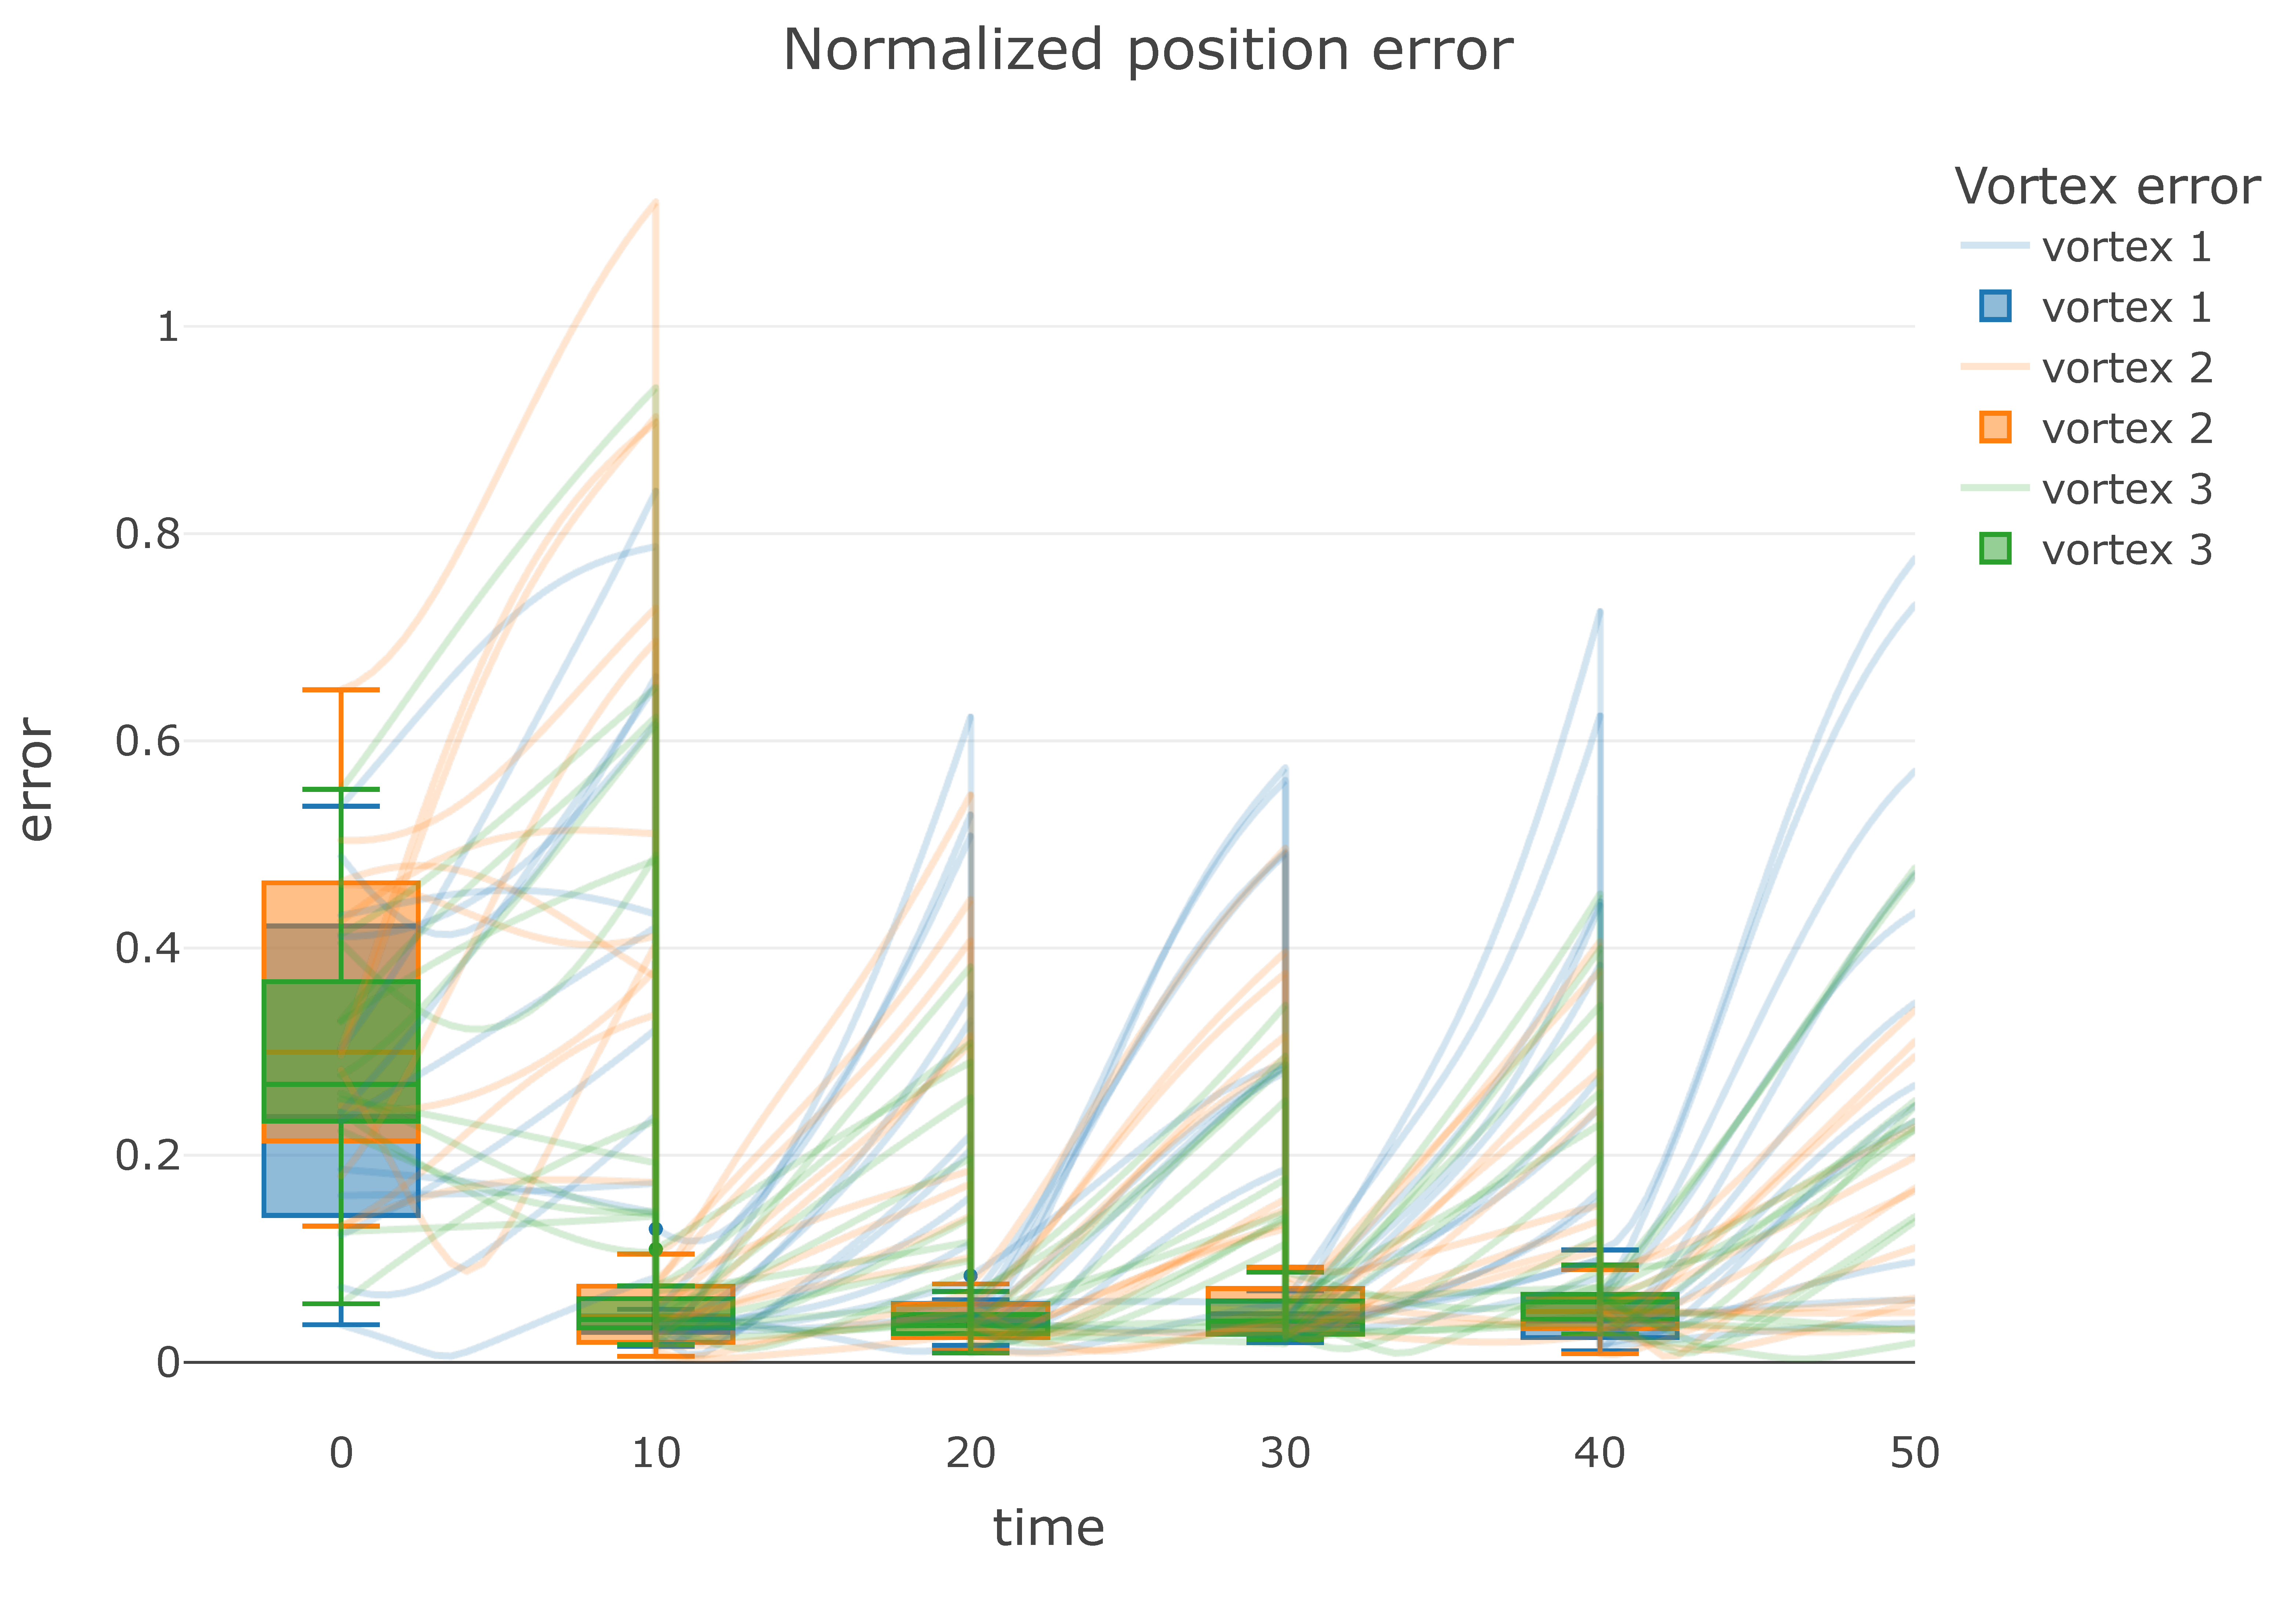
\includegraphics[width=\textwidth]{images/align_error.pdf}
                % \caption*{Vortex position error}
            \end{figure}
            \begin{itemize}
                \item Corrects the position error at each assimilation step
                \item But variability due to uncertainty in strength
            \end{itemize}
        \end{column}
    \end{columns}
\end{frame}

\begin{frame}{Alignment/Strength correction}
    \vspace{-0.5cm}
    \begin{columns}
        \begin{column}{0.5\textwidth}
            \begin{figure}
                \centering
                \animategraphics[loop, autoplay, width=\textwidth]{10}{images/vortex_centers_part_align/vortex_centers_}{0}{36}
                % \caption*{Vortex center trajectories}
            \end{figure}

        \end{column}
        \begin{column}{0.5\textwidth}

            \begin{figure}
                \centering
                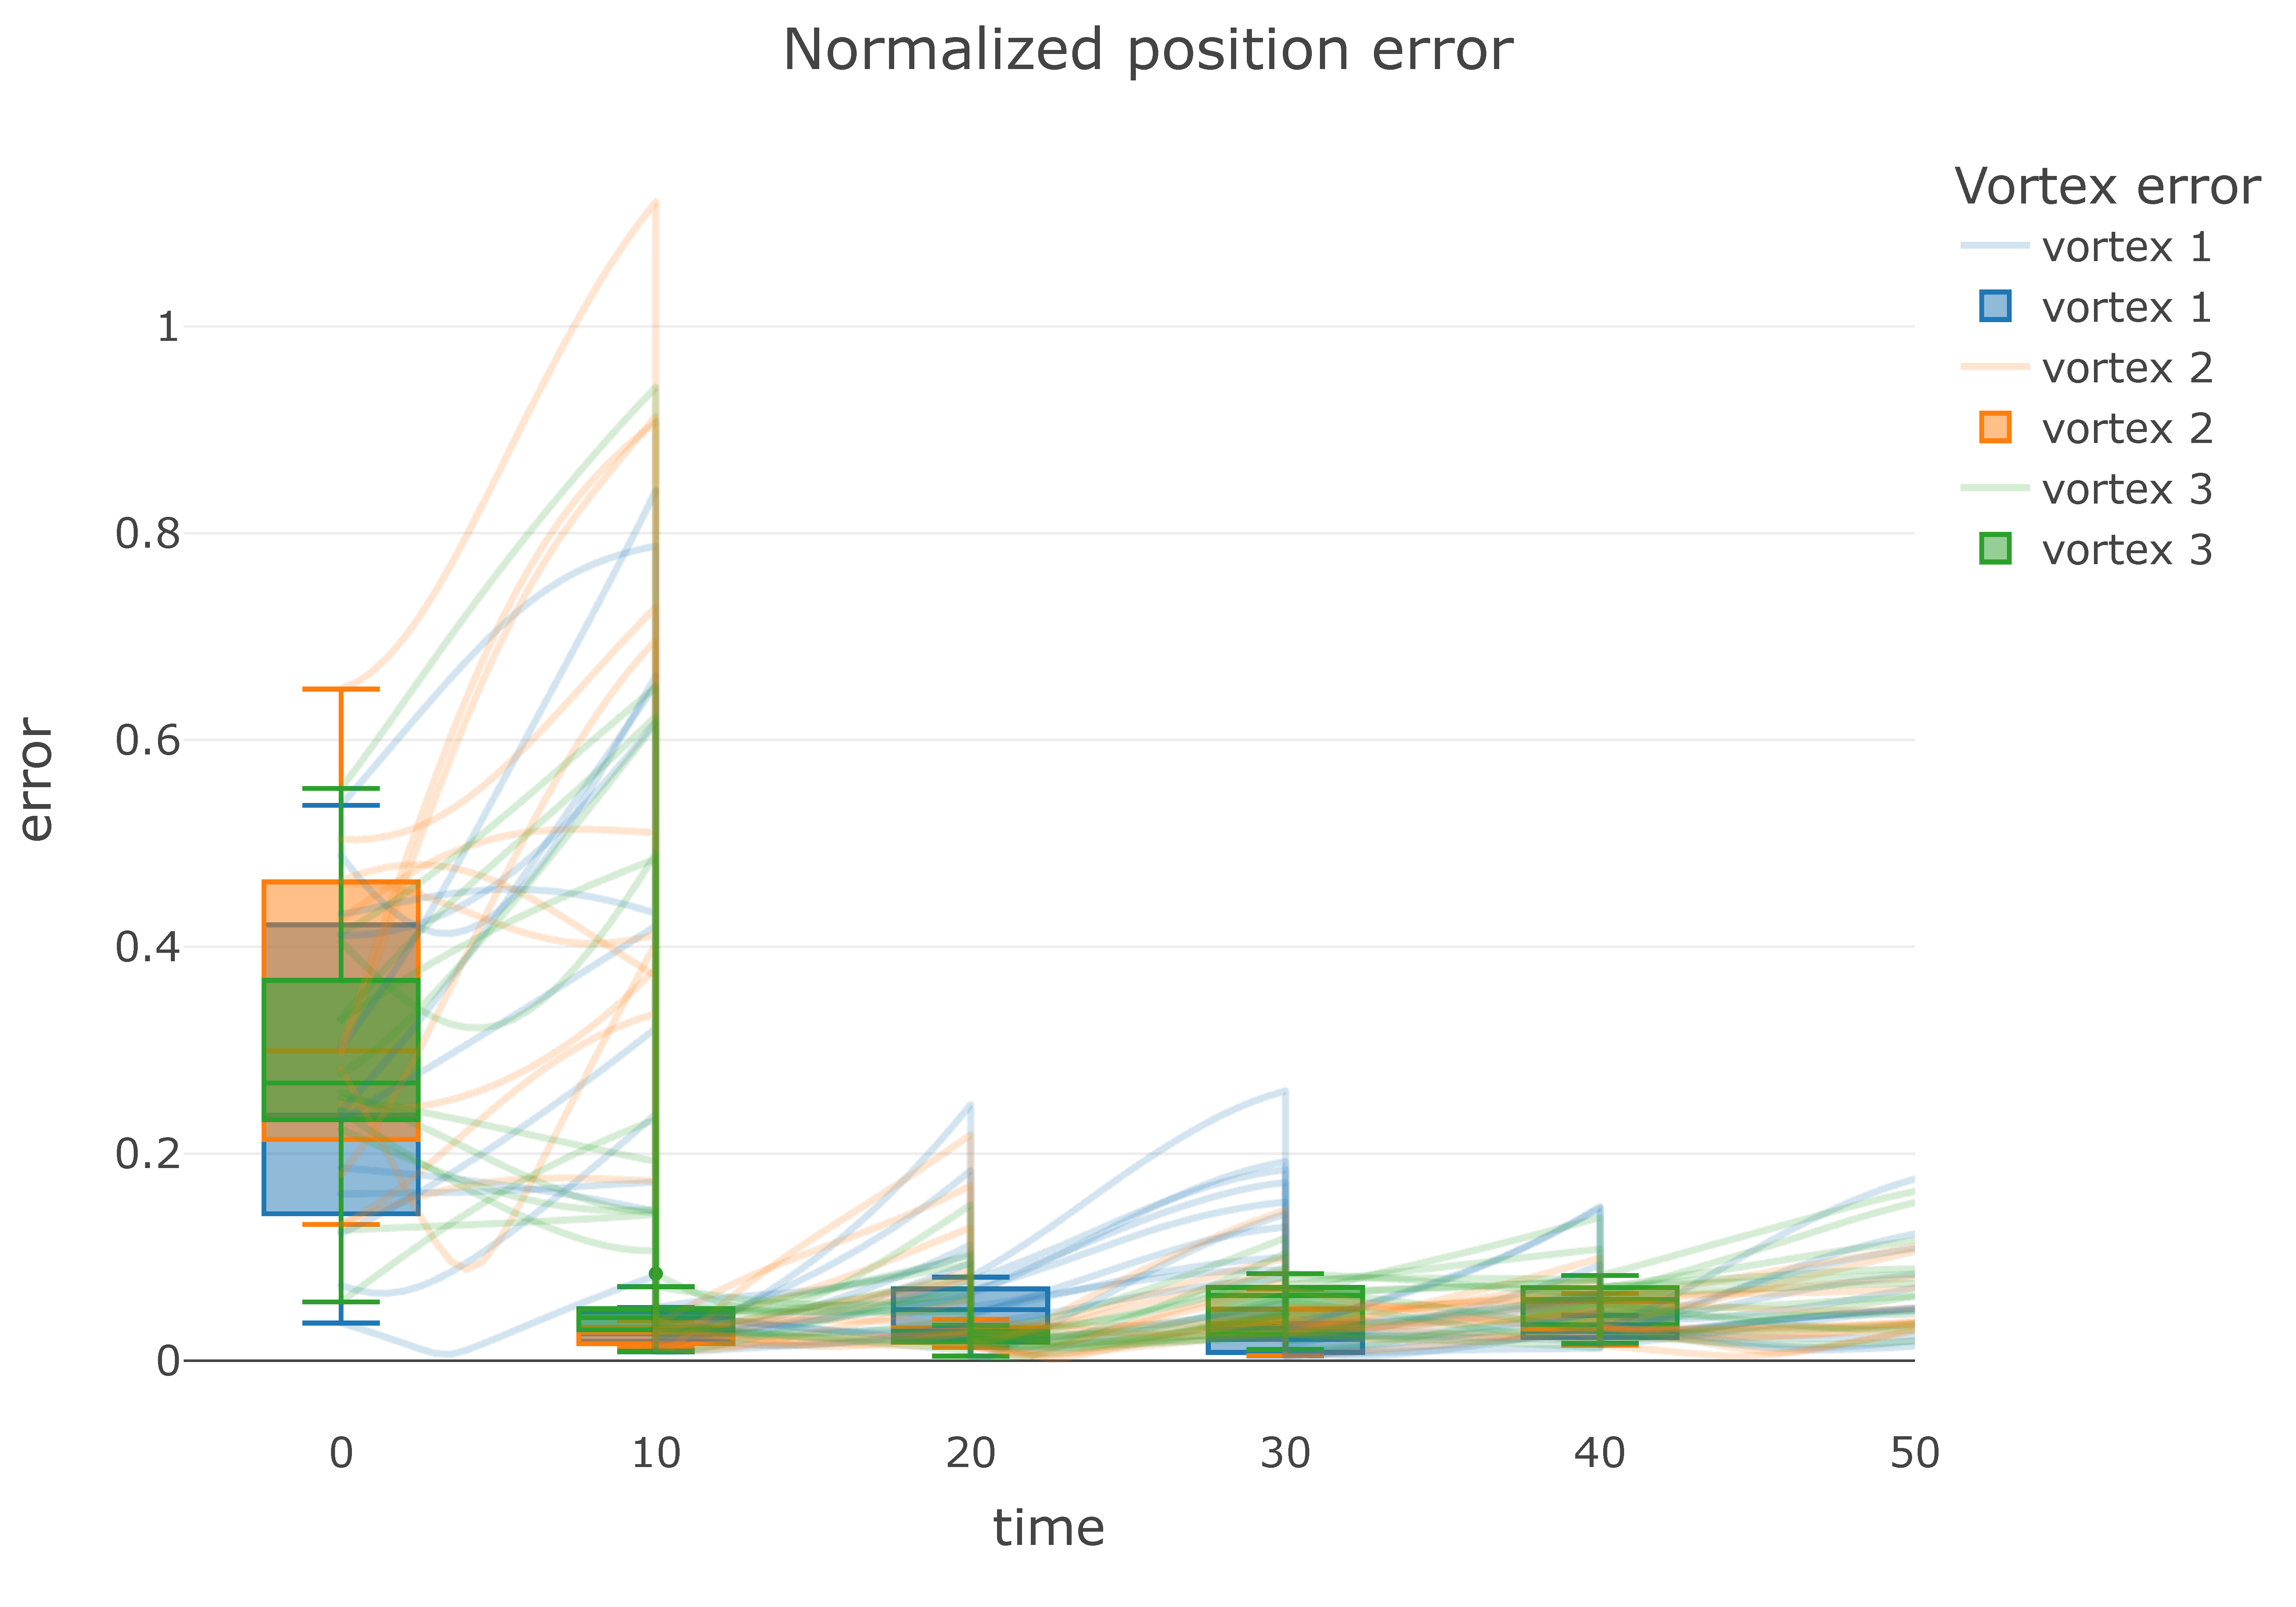
\includegraphics[width=\textwidth]{images/align_part_error.pdf}
            \end{figure}

            \begin{itemize}
                \item Assimilation correct position and reduce strength variability
            \end{itemize}
        \end{column}
    \end{columns}
\end{frame}

\transition[4]{Conclusion}{}
\section{Conclusion}
\begin{frame}{Data assimilation for meshless simulations}{Strength and position correction}

    \begin{itemize}
        \item Improve prediction in the context of meshless simulation
        \item Propose two assimilations approches
              \begin{itemize}
                  \item Strength correction when member discretization overlap
                  \item Position correction to align ensemble of particle sets
                  \item Two methods can be combined
              \end{itemize}
        \item Strength correction is explicit %but computationally intensive
        \item Position correction requires solving a low-dimensional non-linear optimization problem
    \end{itemize}
    \vfill
    \begin{block}{Perspectives}
        \begin{itemize}
            \item Improve computational efficiency
            \item Apply these filters to other meshless modelizations
        \end{itemize}
    \end{block}
\end{frame}

\closingframe

\begin{frame}[allowframebreaks, noframenumbering]
    \frametitle{References}
    \printbibliography % Print the bibliography
\end{frame}

% \section*{Addendum}
% \begin{frame}{EnKF update}
%   \emph{Be successful with your presentation!}
% \end{frame}

\end{document}